% Provenance (never printed): see sources/outline_sources.md (Year 1: fault types and
% Anderson's theory; fold geometry and classification; foliation, schistosity and
% lineation; microstructures). Exercise and problem values in the Book 3 scratch calculator
% calc/ch17.py; the Varden Hills fold and fault from figdata/shared/region.py (read only).
% Fold, anticline, syncline and fold axis are owned by ch. 4; throw and heave by ch. 5;
% trend and plunge by ch. 6; the stresses and the Coulomb criterion by ch. 16. Shear zones
% and deformation mechanisms belong to the Year 3 volume (told here).
\chapter{Faults, Folds and Fabrics}\label{ch:b1:faults-folds-fabrics}

A road cutting shows a rock face polished like glass and scored with fine
parallel grooves. Across the valley, a sea cliff shows beds of sandstone and
shale bent into zigzags with straight sides and sharp corners. On a roof
nearby, slates split into sheets a few millimetres thick, along planes that
cross the layers of the mud they were made from. Each is a record of the
deformation of rock, read at a different scale: the grooves give the direction
in which two blocks slid past each other along a fault; the zigzags measure how
much the beds were shortened; the slaty planes grew across the grain of the rock
as it was squeezed. This chapter gives the geometry needed to measure the three
records, and the mechanics of the previous chapter explains why faults take the
\omterm{def:b1:geological-maps:attitude}{dips} they do.

\begin{recall}
The \omterm{def:b1:geological-maps:attitude}{attitude} of a plane is its \omterm{def:b1:geological-maps:attitude}{dip direction} and \omterm{def:b1:geological-maps:attitude}{dip}, written for instance
$080/12$; its \omterm{def:b1:geological-maps:attitude}{strike} follows by the right-hand rule, the plane dipping to the
right of an observer looking along the \omterm{def:b1:geological-maps:attitude}{strike} (\cref{ch:b1:geological-maps}).
A \omterm{def:b1:geological-maps:fold}{fold} is a bend of once-planar layers; an \omterm{def:b1:geological-maps:fold}{anticline} is convex upward with
the oldest rocks in its core, a \omterm{def:b1:geological-maps:fold}{syncline} concave upward; the \omterm{def:b1:geological-maps:fold}{fold axis} is the
line along which the layers bend most (\cref{ch:b1:geological-maps}). The
\omterm{def:b1:cross-sections:throw}{throw} and \omterm{def:b1:cross-sections:throw}{heave} of a fault are the vertical and horizontal components of its
displacement (\cref{ch:b1:cross-sections}). A line has a \omterm{def:b1:field-lab-methods-1:trend-plunge}{trend} and a \omterm{def:b1:field-lab-methods-1:trend-plunge}{plunge},
and the downward unit vector $(\cos p\sin t, \cos p\cos t, -\sin p)$
(\cref{ch:b1:field-lab-methods-1}). A rock obeying the Coulomb criterion
breaks on planes at $\ang{45} - \phi/2$ from $\sigma_1$, and existing faults
slip according to \omterm{prop:b1:stress-strain-rheology:byerlee}{Byerlee's law} (\cref{ch:b1:stress-strain-rheology}). A
\omterm{def:b1:rock-forming-minerals:mineral}{mineral} is in extinction between \omterm{def:b1:field-lab-methods-1:microscope}{crossed polars} when its vibration directions
are parallel to those of the polars (\cref{ch:b1:optical-mineralogy}). Faults
were met in Book~1, grade~7; \omterm{def:b1:faults-folds-fabrics:fault-types}{reverse faults}, thrusts and \omterm{def:b1:faults-folds-fabrics:foliation}{foliation} in Book~2,
grade~12. The cross product of two vectors is perpendicular to both
(mathematics, Year~1).
\end{recall}

\section{Faults: geometry and kinematics}\label{sec:b1:faults-folds-fabrics:faults}

A fault is a surface across which two blocks of rock have moved past each
other. To describe the movement we need names for the two blocks and for the
displacement, and a way to measure its direction within the plane of the
fault.

\begin{definition}[Hanging wall, footwall, slip vector, net slip, rake]\label{def:b1:faults-folds-fabrics:fault-elements}
Let a fault be locally a plane that is not vertical. The \emph{hanging
wall}\index{hanging wall} is the block above it, the
\emph{footwall}\index{footwall} the block below it. Let $A$ be a point of the
footwall and $A'$ the point of the hanging wall that was in contact with it
before the movement. The \emph{slip vector}\index{slip vector}
$\overrightarrow{AA'}$ is the displacement of the hanging wall relative to the
footwall; its length is the \emph{net slip}\index{net slip}. The
\emph{rake}\index{rake} $r$ (also called the pitch) of the slip vector is the
angle, measured in the plane of the fault, from the \omterm{def:b1:geological-maps:attitude}{strike} direction given by
the right-hand rule to the slip vector, positive when the slip vector points up
the plane and negative when it points down it: $\ang{-180} < r \le \ang{180}$. This is the seismologists'
convention, used again for earthquakes in \cref{ch:b1:earthquake-source}; many
field geologists record instead an angle between 0 and \ang{180}, measured
clockwise from the \omterm{def:b1:geological-maps:attitude}{strike} seen from above, and add the sense of movement in words.
\end{definition}
% ledger: ar:rake, ws:rake, ws:fault-terms

The two names come from mining: a miner working a sloping vein stood on the
\omterm{def:b1:faults-folds-fabrics:fault-elements}{footwall} and had the \omterm{def:b1:faults-folds-fabrics:fault-elements}{hanging wall} over his head. A displacement seen in a
single cut is not, in general, the slip: a bed offset on a map or in a
section shows a separation, which depends on the \omterm{def:b1:geological-maps:attitude}{attitude} of the bed. The slip
needs two points that were once one, such as the two halves of a line cut by
the fault, for instance the edge of a dyke against a bed.

\begin{omfigure}
\begin{tikzpicture}[>={Stealth[length=5pt]}, font=\small]
% (a) the fault plane seen face-on; slip vector of length 3.6 cm at rake -35 deg
% (normal and sinistral): strike-slip component 3.6 cos 35 = 2.949, dip-slip 3.6 sin 35 = 2.065
\pgfmathsetmacro{\Ls}{3.6*cos(35)}\pgfmathsetmacro{\Ld}{3.6*sin(35)}
\begin{scope}
  \fill[omDef!15] (0,0) rectangle (6.2,3.4);
  \draw[omDef, line width=0.7pt] (0,0) rectangle (6.2,3.4);
  \draw[line width=1.2pt] (0,3.4) -- (6.2,3.4);
  \node[anchor=south, font=\scriptsize] at (3.1,3.4) {strike line, where the fault meets the ground};
  \draw[->, line width=0.6pt] (6.45,3.0) -- (6.45,2.0) node[midway, right, font=\scriptsize, align=left] {down\\ the dip};
  \draw[->, line width=0.6pt] (0.3,0.35) -- (1.3,0.35) node[right, font=\scriptsize] {strike};
  \coordinate (A) at (1.2,2.55);
  \coordinate (B) at ($(A)+(\Ls,0)$);
  \coordinate (A2) at ($(A)+(\Ls,-\Ld)$);
  \draw[omProp, dashed, line width=0.7pt] (A) -- (B) node[midway, above, font=\scriptsize] {strike-slip component};
  \draw[omProp, dashed, line width=0.7pt] (B) -- (A2) node[midway, right, font=\scriptsize, align=left] {dip-slip\\ component};
  \draw[->, line width=1.3pt, omThm] (A) -- (A2) node[midway, below left, font=\scriptsize, inner sep=1pt] {slip vector};
  \draw[black] ($(A)+(0.9,0)$) arc[start angle=0, end angle=-35, radius=0.9];
  \node[font=\scriptsize] at ($(A)+(-17.5:1.15)$) {$r$};
  \fill (A) circle[radius=1.4pt] node[above left, inner sep=1.5pt] {$A$};
  \fill (A2) circle[radius=1.4pt] node[below right, inner sep=1.5pt] {$A'$};
  \node[font=\small\bfseries] at (3.1,-0.55) {(a) in the plane of the fault};
\end{scope}
% (b) the vertical section through the dip line: dip 50 deg; dip-slip 2.065 -> throw 1.582, heave 1.327
\begin{scope}[xshift=9.4cm, yshift=0.2cm]
  \pgfmathsetmacro{\th}{\Ld*sin(50)}\pgfmathsetmacro{\he}{\Ld*cos(50)}
  \fill[omLithSand!40] (-1.2,0) -- (-1.2,3.2) -- (0,3.2) -- ({3.2/tan(50)},0) -- cycle;
  \fill[omLithSand!20] ({3.2/tan(50)},0) -- (0,3.2) -- (4.2,3.2) -- (4.2,0) -- cycle;
  \draw[line width=0.6pt] (-1.2,3.2) -- (4.2,3.2);
  \draw[omDef, line width=1.1pt] (0,3.2) -- ({3.2/tan(50)},0);
  \draw[black] (0.75,3.2) arc[start angle=0, end angle=-50, radius=0.75];
  \node[font=\scriptsize] at ($(0,3.2)+(-25:1.0)$) {$\delta$};
  \coordinate (P) at ({1.3*cos(50)},{3.2-1.3*sin(50)});
  \coordinate (Q) at ($(P)+({\Ld*cos(50)},{-\Ld*sin(50)})$);
  \coordinate (R) at ($(P)+(\he,0)$);
  \draw[->, omProp, line width=1.1pt] (P) -- (Q);
  \draw[black!80, densely dotted, line width=0.7pt] (P) -- (R) node[midway, above, font=\scriptsize] {heave};
  \draw[black!80, densely dotted, line width=0.7pt] (R) -- (Q) node[midway, right, font=\scriptsize] {throw};
  \node[font=\scriptsize, omProp, anchor=east] at ($(P)!0.55!(Q)+(-0.08,0)$) {dip slip};
  \node[font=\small] at (3.3,2.6) {hanging wall};
  \node[font=\small] at (-0.55,1.0) {footwall};
  \node[font=\small\bfseries] at (1.5,-0.75) {(b) in the vertical plane of the dip};
\end{scope}
\end{tikzpicture}
\par\smallskip{\small The elements of a fault, drawn to scale for a fault
dipping $\delta = \ang{50}$ and a \omterm{def:b1:faults-folds-fabrics:fault-elements}{slip vector} of \omterm{def:b1:faults-folds-fabrics:fault-elements}{rake} $r = \ang{-35}$. (a) The
fault plane seen face-on: the \omterm{def:b1:faults-folds-fabrics:fault-elements}{slip vector} $\overrightarrow{AA'}$ splits into a
component along the \omterm{def:b1:geological-maps:attitude}{strike} and one down the \omterm{def:b1:geological-maps:attitude}{dip}. (b) The vertical section
perpendicular to the \omterm{def:b1:geological-maps:attitude}{strike}: the dip-slip component splits into the \omterm{def:b1:cross-sections:throw}{throw}
and the \omterm{def:b1:cross-sections:throw}{heave}.}
\label{fig:b1:faults-folds-fabrics:elements}
\end{omfigure}

\begin{proposition}[Components of the slip]\label{prop:b1:faults-folds-fabrics:slip-components}
Let a fault have \omterm{def:b1:geological-maps:attitude}{dip direction} $\alpha$ and \omterm{def:b1:geological-maps:attitude}{dip} $\delta$, and a \omterm{def:b1:faults-folds-fabrics:fault-elements}{slip vector} of
length $L$ and \omterm{def:b1:faults-folds-fabrics:fault-elements}{rake} $r$. With east, north and up components, let
$\mathbf s = (\sin(\alpha-\ang{90}), \cos(\alpha-\ang{90}), 0)$ be the unit
vector along the \omterm{def:b1:geological-maps:attitude}{strike} and $\mathbf u = (-\cos\delta\sin\alpha,
-\cos\delta\cos\alpha, \sin\delta)$ the unit vector up the \omterm{def:b1:geological-maps:attitude}{dip}. Then
\[
  \overrightarrow{AA'} = L\,(\cos r\,\mathbf s + \sin r\,\mathbf u),
\]
its strike-slip component is $L\cos r$ and its dip-slip component $L\sin r$;
the \omterm{def:b1:cross-sections:throw}{throw} is $L\,|\sin r|\sin\delta$, the \omterm{def:b1:cross-sections:throw}{heave} $L\,|\sin r|\cos\delta$, and
the \omterm{def:b1:faults-folds-fabrics:fault-elements}{slip vector} \omterm{def:b1:field-lab-methods-1:trend-plunge}{plunges} by $p$ with $\sin p = |\sin r|\sin\delta$.
\end{proposition}

\begin{proof}
The vector $\mathbf s$ is horizontal and points along the \omterm{def:b1:geological-maps:attitude}{strike}; $\mathbf u$
is the opposite of the downward unit vector of the \omterm{def:b1:geological-maps:attitude}{dip} line, which has \omterm{def:b1:field-lab-methods-1:trend-plunge}{trend}
$\alpha$ and \omterm{def:b1:field-lab-methods-1:trend-plunge}{plunge} $\delta$ (\cref{ch:b1:field-lab-methods-1}). Both lie in
the fault plane, and $\mathbf s\cdot\mathbf u = -\cos\delta(\sin(\alpha -
\ang{90})\sin\alpha + \cos(\alpha - \ang{90})\cos\alpha) = -\cos\delta\cos\ang{90} = 0$,
so they form an orthonormal basis of the plane. A vector of the plane of
length $L$ at the angle $r$ from $\mathbf s$, counted toward $\mathbf u$, is
$L(\cos r\,\mathbf s + \sin r\,\mathbf u)$. Its vertical component is
$L\sin r\sin\delta$, whose size is the \omterm{def:b1:cross-sections:throw}{throw}; its horizontal part across the
\omterm{def:b1:geological-maps:attitude}{strike} is $L\sin r$ times the horizontal part of $\mathbf u$, of length
$\cos\delta$, which is the \omterm{def:b1:cross-sections:throw}{heave}; and the sine of its \omterm{def:b1:field-lab-methods-1:trend-plunge}{plunge} is its vertical
component divided by $L$.
\end{proof}

For a dip-slip fault, $|\sin r| = 1$ and the \omterm{def:b1:cross-sections:throw}{heave} is the \omterm{def:b1:cross-sections:throw}{throw} divided by
$\tan\delta$, as in \cref{ch:b1:cross-sections}. The \omterm{def:b1:faults-folds-fabrics:fault-elements}{rake} sorts faults into
families.

\begin{definition}[Normal, reverse, thrust, strike-slip and oblique-slip faults]\label{def:b1:faults-folds-fabrics:fault-types}
A fault whose \omterm{def:b1:faults-folds-fabrics:fault-elements}{slip vector} lies along the \omterm{def:b1:geological-maps:attitude}{dip} line ($r = \pm\ang{90}$) is a
dip-slip fault: a \emph{normal fault}\index{normal fault} when the \omterm{def:b1:faults-folds-fabrics:fault-elements}{hanging
wall} has moved down ($r = \ang{-90}$), a \emph{reverse fault}\index{reverse
fault} when it has moved up ($r = \ang{90}$). A \emph{thrust
fault}\index{thrust fault} is a reverse fault that \omterm{def:b1:geological-maps:attitude}{dips} \ang{45} or less.
A fault whose slip is parallel to its \omterm{def:b1:geological-maps:attitude}{strike} ($r = 0$ or \ang{180}) is a
\emph{strike-slip fault}\index{strike-slip fault}; such faults are usually
near vertical. A strike-slip fault is \emph{dextral}\index{dextral}
(right-lateral) when an observer standing on one side sees the other side
moved to the right, \emph{sinistral}\index{sinistral} (left-lateral) when to
the left. A fault whose slip has both a strike-slip and a dip-slip component
is an \emph{oblique-slip fault}\index{oblique-slip fault}; in practice a
fault is named after its larger component, so that a \omterm{def:b1:faults-folds-fabrics:fault-elements}{rake} near \ang{-90} is
called normal.
\end{definition}
% ledger: usgs:fault-types, ws:fault-terms, ar:rake

\begin{proposition}[The sense of a strike-slip fault]\label{prop:b1:faults-folds-fabrics:sense}
The sense of a \omterm{def:b1:faults-folds-fabrics:fault-types}{strike-slip fault} does not depend on the side the observer
stands on. A \omterm{def:b1:faults-folds-fabrics:fault-elements}{rake} near $0$ is \omterm{def:b1:faults-folds-fabrics:fault-types}{sinistral}, a \omterm{def:b1:faults-folds-fabrics:fault-elements}{rake} near \ang{180} \omterm{def:b1:faults-folds-fabrics:fault-types}{dextral}.
\end{proposition}

\begin{proof}
If an observer on block 1 sees block 2 move by $\mathbf v$, an observer on
block 2 sees block 1 move by $-\mathbf v$. Turning round to face block 1, the
second observer has exchanged left and right. The two changes cancel: both
see the other side go the same way, to the right or to the left. For the
second part, stand on the \omterm{def:b1:faults-folds-fabrics:fault-elements}{footwall} and face the \omterm{def:b1:faults-folds-fabrics:fault-elements}{hanging wall}: one then looks
down the \omterm{def:b1:geological-maps:attitude}{dip direction}, and since the plane \omterm{def:b1:geological-maps:attitude}{dips} to the right of its \omterm{def:b1:geological-maps:attitude}{strike},
the \omterm{def:b1:geological-maps:attitude}{strike} direction points to one's left. A \omterm{def:b1:faults-folds-fabrics:fault-elements}{rake} of $0$ moves the \omterm{def:b1:faults-folds-fabrics:fault-elements}{hanging wall}
along the \omterm{def:b1:geological-maps:attitude}{strike}, to the left; a \omterm{def:b1:faults-folds-fabrics:fault-elements}{rake} of \ang{180} moves it to the right.
\end{proof}

A fault surface is often itself a record of the movement: the scratches and
fibres on it lie along the slip. Around the surface, a fault zone may be filled
with rock broken by the movement.

\begin{definition}[Slickenside, slickenlines, fault rocks]\label{def:b1:faults-folds-fabrics:fault-rocks}
\emph{Slickenlines}\index{slickenlines} are scratches or fibres on a fault
surface, parallel to the slip; a \emph{slickenside}\index{slickenside} is a
fault surface that carries them, often smoothed by the slip. A \emph{fault
rock}\index{fault rock} is a rock made by the movement on a fault. A
\emph{fault breccia}\index{fault breccia} is made of angular fragments of the
walls of the fault, rotated and moved out of place, from huge blocks down to
about \qty{2}{mm}; a \emph{cataclasite}\index{cataclasite} is made of
fragments of sand size or smaller; neither has a fabric, the fragments lying
at random. A \emph{fault gouge}\index{fault gouge} is a fault rock rich in
clay, very soft in \omterm{def:b1:geological-maps:geological-map}{outcrop}. A \emph{mylonite}\index{mylonite} is a
fine-grained, strongly foliated rock made in a shear zone by ductile shearing,
the grains shrunk by recrystallisation rather than by milling.
\end{definition}
% ledger: ws:fault-terms, ws:fault-rocks

The \omterm{def:b1:faults-folds-fabrics:fault-rocks}{fault rocks} are a depth gauge, and they follow the \omterm{def:b1:stress-strain-rheology:strength-envelope}{strength envelope} of
\cref{ch:b1:stress-strain-rheology}. Gouge, breccia and \omterm{def:b1:faults-folds-fabrics:fault-rocks}{cataclasite}, with
their random fabric, are made by frictional sliding and fracture in the
brittle \omterm{def:b1:layered-earth:layers}{crust}; \omterm{def:b1:faults-folds-fabrics:fault-rocks}{mylonites} are made below the \omterm{def:b1:stress-strain-rheology:strength-envelope}{brittle--ductile transition}, where
the fault continues downward as a band of ductile shear. For a normal
\omterm{def:b1:heat-budget:geotherm}{geotherm} and enough water, the transition between the two lies at
\qtyrange{10}{15}{km}, close to the \qty{13.7}{km} of the envelope of the
previous chapter, and the fault is strongest there. Across a large fault
brought up from depth, the same order is found side by side: gouge zones near
the surface, then \omterm{def:b1:faults-folds-fabrics:fault-rocks}{cataclasite}, then \omterm{def:b1:faults-folds-fabrics:fault-rocks}{mylonite}.
The name \omterm{def:b1:faults-folds-fabrics:fault-rocks}{mylonite}, from the Greek word for milling flour, records a mistake:
it was thought to be ground rock. The Year~3 volume studies those deep shear
zones and the mechanisms that make \omterm{def:b1:faults-folds-fabrics:fault-rocks}{mylonites}.
% ledger: sibson:fault-rocks, sibson:alpine-fault, ws:fault-rocks

\begin{omfigure}
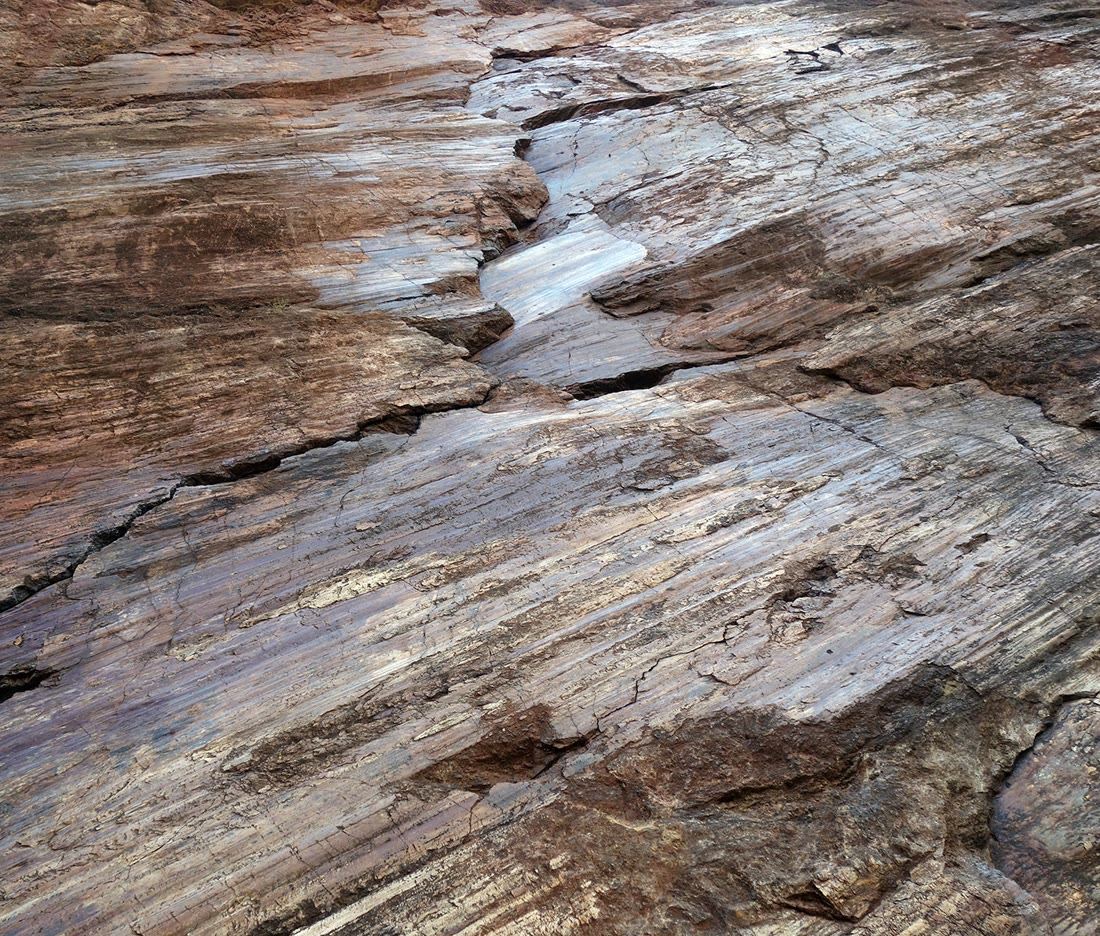
\includegraphics[height=5.2cm]{images/book3/b1-slickenside.jpg}\hfill
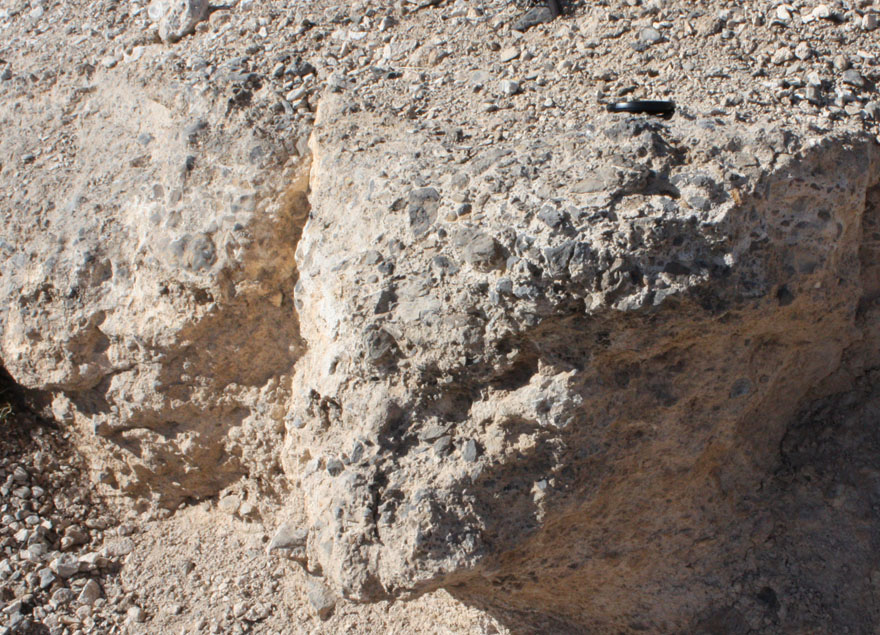
\includegraphics[height=5.2cm]{images/book3/b1-fault-breccia.jpg}
\par\smallskip{\small Left: a \omterm{def:b1:faults-folds-fabrics:fault-rocks}{slickenside} on a fault surface in chert, about
\qtyproduct{3 x 3}{m} of a surface \qty{10}{m} high, Corona Heights, San
Francisco; the polished face is striated along the slip. Photograph:
Dextersinister, CC~BY-SA~4.0. Right: \omterm{def:b1:faults-folds-fabrics:fault-rocks}{fault breccia} of the Keystone Thrust, Red
Rock Canyon, Nevada: angular fragments of grey carbonate rock in a paler
matrix; the lens cap at the top right is \qty{5.8}{cm} across. Photograph:
Jstuby, public domain. Both from Wikimedia Commons.}
\label{fig:b1:faults-folds-fabrics:fault-surfaces}
\end{omfigure}
% ledger: commons:slickenside, commons:breccia

\begin{method}[Measuring the slip on a fault]\label{met:b1:faults-folds-fabrics:slip}
\begin{enumerate}
  \item Measure the \omterm{def:b1:geological-maps:attitude}{attitude} $\alpha/\delta$ of the fault surface and write its
        \omterm{def:b1:geological-maps:attitude}{strike}, $\alpha - \ang{90}$.
  \item Measure the \omterm{def:b1:faults-folds-fabrics:fault-rocks}{slickenlines}: their \omterm{def:b1:faults-folds-fabrics:fault-elements}{rake} on the fault, or their \omterm{def:b1:field-lab-methods-1:trend-plunge}{trend} and
        \omterm{def:b1:field-lab-methods-1:trend-plunge}{plunge}; for a \omterm{def:b1:faults-folds-fabrics:fault-elements}{rake} $r$, $\sin p = |\sin r|\sin\delta$.
  \item Find which way the \omterm{def:b1:faults-folds-fabrics:fault-elements}{hanging wall} moved, from markers offset across the
        fault, and give the \omterm{def:b1:faults-folds-fabrics:fault-elements}{rake} its sign: negative if the \omterm{def:b1:faults-folds-fabrics:fault-elements}{hanging wall} went
        down.
  \item Find the \omterm{def:b1:faults-folds-fabrics:fault-elements}{net slip} $L$ from two points that were once one; if only the
        \omterm{def:b1:cross-sections:throw}{throw} $h$ of a horizontal marker is known, $L = h/(|\sin r|\sin\delta)$.
  \item Compute the components with
        \cref{prop:b1:faults-folds-fabrics:slip-components} and name the fault
        with \cref{def:b1:faults-folds-fabrics:fault-types}.
\end{enumerate}
\end{method}

\begin{inthefield}[Measuring a fault surface]
A geologist who finds a fault surface in an \omterm{def:b1:geological-maps:geological-map}{outcrop} measures it like any other
plane, with a compass-clinometer laid on the surface, and then measures the
\omterm{def:b1:faults-folds-fabrics:fault-rocks}{slickenlines} on it, either as a \omterm{def:b1:faults-folds-fabrics:fault-elements}{rake}, with a protractor laid on the plane, or
as a \omterm{def:b1:field-lab-methods-1:trend-plunge}{trend} and \omterm{def:b1:field-lab-methods-1:trend-plunge}{plunge}. The two are checked against each other with the
formula of step~2 of the method. The sense of movement is the hard part. Small
steps on a \omterm{def:b1:faults-folds-fabrics:fault-rocks}{slickenside}, and fibres of quartz or calcite that grew as the
blocks moved apart, can show which way the missing block went, but some steps
point the wrong way, so the sense is trusted only when it agrees with the
offset of a marker bed or a vein. \omterm{def:b1:faults-folds-fabrics:fault-rocks}{Fault rocks} are described and sampled, and a
fault zone too broad to measure in one place is mapped as a band. Each fault is
recorded at a numbered station of the notebook, with its \omterm{def:b1:geological-maps:attitude}{attitude}, its
\omterm{def:b1:faults-folds-fabrics:fault-rocks}{slickenlines}, the sense of movement and how sure the geologist is of it.
\end{inthefield}

\section{Anderson's theory of faulting}\label{sec:b1:faults-folds-fabrics:anderson}

Why are most \omterm{def:b1:faults-folds-fabrics:fault-types}{normal faults} steep and most thrusts gentle? In 1905 the Scottish
geologist Ernest Masson Anderson answered with two remarks: the surface of the
Earth fixes the directions of the \omterm{def:b1:stress-strain-rheology:principal}{principal stresses}, and the Coulomb
criterion then fixes the angle of the faults.
% ledger: ws:anderson, anderson:1905

\begin{proposition}[A free surface makes a principal plane]\label{prop:b1:faults-folds-fabrics:free-surface}
At the surface of the Earth, where it is horizontal, one principal stress is
vertical and the other two are horizontal.
\end{proposition}

\begin{proof}
The air presses on the ground only with its pressure, normal to the surface:
it exerts no shear stress. The stress on the horizontal plane at the surface
is therefore normal to it. In three dimensions, the stress on a plane of unit
normal $\mathbf n$ is the vector $\boldsymbol\sigma\mathbf n$ (physics books,
Year~3); if it has no shear part, it is parallel to $\mathbf n$, so that
$\boldsymbol\sigma\mathbf n = \lambda\mathbf n$ and $\mathbf n$ is an
eigenvector of the symmetric matrix $\boldsymbol\sigma$: a principal
direction (\cref{def:b1:stress-strain-rheology:principal}). The vertical is
thus a principal direction, and the two others, perpendicular to it, are
horizontal.
\end{proof}

Anderson assumed that the \omterm{def:b1:stress-strain-rheology:principal}{principal stresses} keep these directions down to
the depths at which faults form. The assumption holds well under a gently
sloping surface and in rocks without strong old weaknesses; it fails near
steep relief and where old faults or layers guide the new ones. With it, only
three cases are possible, according to which of $\sigma_1$, $\sigma_2$ and
$\sigma_3$ is vertical.

\begin{theorem}[Anderson's theory of faulting]\label{thm:b1:faults-folds-fabrics:anderson}
Let one principal stress be vertical and let the rock break according to the
Coulomb criterion, with \omterm{def:b1:stress-strain-rheology:coulomb}{angle of internal friction} $\phi$. New faults form on
planes that contain the direction of $\sigma_2$ and make the angle
$\ang{45} - \phi/2$ with $\sigma_1$, and they slip perpendicular to $\sigma_2$,
shortening the rock along $\sigma_1$. Hence
\begin{enumerate}[label=(\alph*)]
  \item if $\sigma_1$ is vertical, \omterm{def:b1:faults-folds-fabrics:fault-types}{normal faults} form, striking along
        $\sigma_2$ and dipping $\ang{45} + \phi/2$;
  \item if $\sigma_3$ is vertical, \omterm{def:b1:faults-folds-fabrics:fault-types}{thrust faults} form, striking along
        $\sigma_2$ and dipping $\ang{45} - \phi/2$;
  \item if $\sigma_2$ is vertical, vertical \omterm{def:b1:faults-folds-fabrics:fault-types}{strike-slip faults} form, striking
        at $\ang{45} - \phi/2$ on either side of $\sigma_1$.
\end{enumerate}
With $\phi = \ang{30}$, the \omterm{def:b1:geological-maps:attitude}{dips} are \ang{60}, \ang{30} and \ang{90}.
\end{theorem}
\index{Anderson's theory of faulting}

\begin{proof}
On a plane that contains the direction of $\sigma_2$, the normal lies in the
plane of $\sigma_1$ and $\sigma_3$, and the stress on the plane is that of the
two-dimensional problem of \cref{ch:b1:stress-strain-rheology}: its point
lies on the Mohr circle of $\sigma_1$ and $\sigma_3$, and its shear part lies
in the plane of $\sigma_1$ and $\sigma_3$, perpendicular to $\sigma_2$. On any
other plane, the point $(\sigma_n, \tau)$ lies inside that circle, which is
the largest of the three Mohr circles of a three-dimensional state of stress
(admitted from the three-dimensional theory). As the stresses grow, the Coulomb
line is therefore first touched by planes containing $\sigma_2$, and among
them, by \cref{thm:b1:stress-strain-rheology:failure-angle}, by those at
$\ang{45} - \phi/2$ from $\sigma_1$. Slip on such a plane, perpendicular to
$\sigma_2$, brings closer the two blocks along the direction of greatest
compression and moves them apart along the least, as it must to relieve the
stress. In case (a) the plane makes the angle $\ang{45} - \phi/2$ with the
vertical, so it \omterm{def:b1:geological-maps:attitude}{dips} $\ang{45} + \phi/2$; it \omterm{def:b1:geological-maps:attitude}{strikes} along the horizontal
$\sigma_2$; the slip lies in the vertical plane of the \omterm{def:b1:geological-maps:attitude}{dip}, and the block above
goes down, lengthening the rock horizontally: a \omterm{def:b1:faults-folds-fabrics:fault-types}{normal fault}. In case (b) the
plane makes $\ang{45} - \phi/2 < \ang{45}$ with the horizontal $\sigma_1$, and
the slip shortens the rock horizontally, pushing the \omterm{def:b1:faults-folds-fabrics:fault-elements}{hanging wall} up: a
\omterm{def:b1:faults-folds-fabrics:fault-types}{thrust fault}. In case (c) the planes contain the vertical, so they are
vertical; the slip is horizontal, perpendicular to $\sigma_2$: \omterm{def:b1:faults-folds-fabrics:fault-types}{strike-slip
faults}, at $\ang{45} - \phi/2$ on either side of the horizontal $\sigma_1$.
\end{proof}

In each regime two sets of faults are possible, symmetric about $\sigma_1$:
conjugate faults, meeting at $\ang{90} - \phi$, about \ang{60}, with
$\sigma_1$ in the acute angle between them. Conversely, a pair of conjugate
faults measured in the field gives the directions of the stresses that made
them: $\sigma_1$ bisects their acute angle, $\sigma_2$ is their line of
intersection.

\begin{omfigure}
\begin{tikzpicture}[x={(1cm,0cm)}, y={(0.42cm,0.30cm)}, z={(0cm,1cm)},
  >={Stealth[length=5pt]}, font=\small, scale=0.86,
  face/.style={draw=black, line width=0.5pt, line join=round},
  sone/.style={->, line width=1.6pt, omThm},
  sthree/.style={->, line width=0.8pt, omDef}]
% exact geometry: the fault plane is X = xf(Z); slip is along the dip; throw t
% (a) normal fault: dip 60, xf(Z) = 1.3 + (1.6 - Z)/tan 60, throw 0.45
\begin{scope}
  \def\W{3.2}\def\D{1.6}\def\H{1.6}
  \pgfmathsetmacro{\c}{1/tan(60)}
  \pgfmathsetmacro{\xa}{1.3+1.6*\c}       % xf(0)
  \pgfmathsetmacro{\xb}{1.3+0.45*\c}      % xf(H - t)
  \pgfmathsetmacro{\mfa}{1.3+(1.6-0.55)*\c}\pgfmathsetmacro{\mfb}{1.3+(1.6-0.85)*\c}
  \pgfmathsetmacro{\mha}{1.3+(1.6-0.10)*\c}\pgfmathsetmacro{\mhb}{1.3+(1.6-0.40)*\c}
  % footwall
  \fill[omLithSand!55] (0,0,0) -- (\xa,0,0) -- (1.3,0,\H) -- (0,0,\H) -- cycle;
  \fill[omProp!40] (0,0,0.55) -- (\mfa,0,0.55) -- (\mfb,0,0.85) -- (0,0,0.85) -- cycle;
  \draw[face] (0,0,0) -- (\xa,0,0) -- (1.3,0,\H) -- (0,0,\H) -- cycle;
  \draw[face, fill=omLithSand!35] (0,0,\H) -- (1.3,0,\H) -- (1.3,\D,\H) -- (0,\D,\H) -- cycle;
  \draw[face, fill=black!12] (1.3,0,\H) -- (\xb,0,1.15) -- (\xb,\D,1.15) -- (1.3,\D,\H) -- cycle;
  % hanging wall
  \fill[omLithSand!55] (\xa,0,0) -- (\W,0,0) -- (\W,0,1.15) -- (\xb,0,1.15) -- cycle;
  \fill[omProp!40] (\mha,0,0.10) -- (\W,0,0.10) -- (\W,0,0.40) -- (\mhb,0,0.40) -- cycle;
  \draw[face] (\xa,0,0) -- (\W,0,0) -- (\W,0,1.15) -- (\xb,0,1.15) -- cycle;
  \draw[face, fill=omLithSand!35] (\xb,0,1.15) -- (\W,0,1.15) -- (\W,\D,1.15) -- (\xb,\D,1.15) -- cycle;
  \fill[omLithSand!45] (\W,0,0) -- (\W,\D,0) -- (\W,\D,1.15) -- (\W,0,1.15) -- cycle;
  \fill[omProp!30] (\W,0,0.10) -- (\W,\D,0.10) -- (\W,\D,0.40) -- (\W,0,0.40) -- cycle;
  \draw[face] (\W,0,0) -- (\W,\D,0) -- (\W,\D,1.15) -- (\W,0,1.15) -- cycle;
  % slip arrow on the front face
  \draw[->, line width=0.9pt] (1.45,0,1.05) -- ++({0.35*cos(60)},0,{-0.35*sin(60)});
  % stresses: sigma1 vertical, sigma3 horizontal across the strike
  \draw[sone] (1.6,0.8,3.05) -- (1.6,0.8,2.1) node[pos=0, left] {$\sigma_1$};
  \draw[sone] (1.6,0.8,-1.1) -- (1.6,0.8,-0.15);
  \draw[sthree] (-0.85,0.8,0.8) -- (-0.15,0.8,0.8) node[pos=0, above] {$\sigma_3$};
  \draw[sthree] (4.05,0.8,0.6) -- (3.35,0.8,0.6);
  \node[font=\small\bfseries] at (1.9,0,-1.55) {(a) normal fault};
\end{scope}
% (b) thrust fault: dip 30, xf(Z) = 3.0 - Z/tan 30, throw 0.35, heave 0.606
\begin{scope}[xshift=6.0cm]
  \def\D{1.6}\def\H{1.3}
  \pgfmathsetmacro{\c}{1/tan(30)}
  \pgfmathsetmacro{\Wp}{4.0-0.35*\c}       % right face of the hanging wall
  \pgfmathsetmacro{\xt}{3.0-1.3*\c}        % footwall top edge
  \pgfmathsetmacro{\xh}{3.0-1.65*\c}       % hanging-wall top edge
  \pgfmathsetmacro{\mfa}{3.0-0.50*\c}\pgfmathsetmacro{\mfb}{3.0-0.75*\c}
  \pgfmathsetmacro{\mha}{3.0-0.85*\c}\pgfmathsetmacro{\mhb}{3.0-1.10*\c}
  % footwall
  \fill[omLithSand!55] (0,0,0) -- (3.0,0,0) -- (\xt,0,\H) -- (0,0,\H) -- cycle;
  \fill[omProp!40] (0,0,0.50) -- (\mfa,0,0.50) -- (\mfb,0,0.75) -- (0,0,0.75) -- cycle;
  \draw[face] (0,0,0) -- (3.0,0,0) -- (\xt,0,\H) -- (0,0,\H) -- cycle;
  \draw[face, fill=omLithSand!35] (0,0,\H) -- (\xt,0,\H) -- (\xt,\D,\H) -- (0,\D,\H) -- cycle;
  % hanging wall
  \fill[omLithSand!55] (3.0,0,0) -- (\Wp,0,0) -- (\Wp,0,1.65) -- (\xh,0,1.65) -- cycle;
  \fill[omProp!40] (\mha,0,0.85) -- (\Wp,0,0.85) -- (\Wp,0,1.10) -- (\mhb,0,1.10) -- cycle;
  \draw[face] (3.0,0,0) -- (\Wp,0,0) -- (\Wp,0,1.65) -- (\xh,0,1.65) -- cycle;
  \draw[face, fill=omLithSand!35] (\xh,0,1.65) -- (\Wp,0,1.65) -- (\Wp,\D,1.65) -- (\xh,\D,1.65) -- cycle;
  \fill[omLithSand!45] (\Wp,0,0) -- (\Wp,\D,0) -- (\Wp,\D,1.65) -- (\Wp,0,1.65) -- cycle;
  \fill[omProp!30] (\Wp,0,0.85) -- (\Wp,\D,0.85) -- (\Wp,\D,1.10) -- (\Wp,0,1.10) -- cycle;
  \draw[face] (\Wp,0,0) -- (\Wp,\D,0) -- (\Wp,\D,1.65) -- (\Wp,0,1.65) -- cycle;
  \draw[->, line width=0.9pt] (2.25,0,0.62) -- ++({-0.42*cos(30)},0,{0.42*sin(30)});
  % stresses: sigma1 horizontal across the strike, sigma3 vertical
  \draw[sone] (-1.2,0.8,0.65) -- (-0.15,0.8,0.65) node[pos=0, above] {$\sigma_1$};
  \draw[sone] (\Wp+1.15,0.8,0.45) -- (\Wp+0.1,0.8,0.45);
  \draw[sthree] (2.0,0.8,2.7) -- (2.0,0.8,2.0) node[pos=0, left] {$\sigma_3$};
  \draw[sthree] (2.0,0.8,-0.9) -- (2.0,0.8,-0.2);
  \node[font=\small\bfseries] at (2.0,0,-1.55) {(b) thrust fault};
\end{scope}
% (c) strike-slip fault: vertical, along the y axis at X = 1.6; dextral: the far
% (east) block has moved toward the reader by 0.5; sigma1 at 30 deg clockwise of the strike
\begin{scope}[xshift=12.0cm]
  \def\D{2.2}\def\H{1.1}\def\s{0.5}
  % west block
  \draw[face, fill=omLithSand!55] (0,0,0) -- (1.6,0,0) -- (1.6,0,\H) -- (0,0,\H) -- cycle;
  \draw[face, fill=omLithSand!35] (0,0,\H) -- (1.6,0,\H) -- (1.6,\D,\H) -- (0,\D,\H) -- cycle;
  \draw[face, fill=black!12] (1.6,\D-\s,0) -- (1.6,\D,0) -- (1.6,\D,\H) -- (1.6,\D-\s,\H) -- cycle;
  \draw[line width=1.4pt, omProp] (0,1.25,\H) -- (1.6,1.25,\H);
  % east block
  \draw[face, fill=omLithSand!55] (1.6,-\s,0) -- (3.2,-\s,0) -- (3.2,-\s,\H) -- (1.6,-\s,\H) -- cycle;
  \draw[face, fill=omLithSand!35] (1.6,-\s,\H) -- (3.2,-\s,\H) -- (3.2,\D-\s,\H) -- (1.6,\D-\s,\H) -- cycle;
  \draw[face, fill=omLithSand!45] (3.2,-\s,0) -- (3.2,\D-\s,0) -- (3.2,\D-\s,\H) -- (3.2,-\s,\H) -- cycle;
  \draw[line width=1.4pt, omProp] (1.6,1.25-\s,\H) -- (3.2,1.25-\s,\H);
  % slip arrows on the top
  \draw[->, line width=0.9pt] (2.05,1.35,\H) -- (2.05,0.35,\H);
  \draw[->, line width=0.9pt] (1.15,0.55,\H) -- (1.15,1.55,\H);
  % stresses in the horizontal plane, drawn at the height of the top surface
  \draw[sone] ({1.6+1.9*sin(30)},{0.8+1.9*cos(30)},\H) -- ({1.6+1.0*sin(30)},{0.8+1.0*cos(30)},\H) node[pos=0, right] {$\sigma_1$};
  \draw[sone] ({1.6-1.9*sin(30)},{0.8-1.9*cos(30)},\H) -- ({1.6-1.0*sin(30)},{0.8-1.0*cos(30)},\H);
  \draw[sthree] ({1.6+2.0*sin(120)},{0.8+2.0*cos(120)},\H) -- ({1.6+1.45*sin(120)},{0.8+1.45*cos(120)},\H) node[pos=0, right] {$\sigma_3$};
  \draw[sthree] ({1.6-2.0*sin(120)},{0.8-2.0*cos(120)},\H) -- ({1.6-1.45*sin(120)},{0.8-1.45*cos(120)},\H);
  \node[font=\small\bfseries] at (1.7,0,-1.55) {(c) strike-slip fault};
\end{scope}
\end{tikzpicture}
\par\smallskip{\small Anderson's three regimes, with the faults at the \omterm{def:b1:geological-maps:attitude}{dips}
of the theorem for $\phi = \ang{30}$: \ang{60}, \ang{30} and vertical. Thick
red arrows: $\sigma_1$; thin blue arrows: $\sigma_3$; $\sigma_2$ runs along
the \omterm{def:b1:geological-maps:attitude}{strike} of the faults in (a) and (b) and is vertical in (c). A marker bed
(orange) is offset by the \omterm{def:b1:cross-sections:throw}{throw} in (a) and (b); in (c) a line on the ground is
offset horizontally, and the fault is \omterm{def:b1:faults-folds-fabrics:fault-types}{dextral}: seen from either block, the
other has moved to the right. The black arrows give the slip.}
\label{fig:b1:faults-folds-fabrics:anderson}
\end{omfigure}

The three regimes match the three kinds of plate boundary of
\cref{ch:b1:rifts-ridges-margins,ch:b1:active-margins}. Where the \omterm{def:b1:layered-earth:lithosphere}{lithosphere}
is stretched, at rifts and ridges, the horizontal stress falls below the
vertical one and \omterm{def:b1:faults-folds-fabrics:fault-types}{normal faults} form; where it is squeezed, at convergent
margins and in mountain belts, the horizontal stress exceeds the weight of the
rock and thrusts form; along \omterm{def:b1:rifts-ridges-margins:transform}{transform faults} the two horizontal stresses
straddle the vertical one. The \omterm{def:b1:geological-maps:attitude}{dips} fit the observations in a rough way: the
\omterm{def:b1:faults-folds-fabrics:fault-types}{normal faults} of rifts \omterm{def:b1:geological-maps:attitude}{dip} around \ang{60} near the surface, and thrusts are
low-angle \omterm{def:b1:faults-folds-fabrics:fault-types}{reverse faults}. The exceptions are informative. Many \omterm{def:b1:faults-folds-fabrics:fault-types}{normal faults}
flatten with depth, and some cross-sections of rifts show them reaching a
nearly flat zone of shear: these low-angle \omterm{def:b1:faults-folds-fabrics:fault-types}{normal faults}, or detachments, cut
the \omterm{def:b1:layered-earth:layers}{crust} at well under \ang{45}. Anderson's theory cannot explain
them as new faults, and \cref{exo:b1:faults-folds-fabrics:10} shows that
Byerlee's friction cannot make them slip under Andersonian stresses either:
they need weak \omterm{def:b1:faults-folds-fabrics:fault-rocks}{fault rocks}, high pore pressure or rotated stresses. A fault
that already exists slips at the friction of \omterm{prop:b1:stress-strain-rheology:byerlee}{Byerlee's law},
$\mu = 0.85$, $\phi = \ang{40.4}$; the best-oriented \omterm{def:b1:faults-folds-fabrics:fault-types}{normal faults} then \omterm{def:b1:geological-maps:attitude}{dip}
\ang{65.2}, as the problem of \cref{ch:b1:stress-strain-rheology} found.
% ledger: ws:anderson, usgs:fault-types, byerlee:1975

\begin{history}[Anderson's faults]
Ernest Masson Anderson, a Scottish geologist, published his theory of the
three kinds of faults in 1905, in a short paper on the dynamics of faulting,
and gave its full form, with its application to the dykes and faults of
Britain, in his book \emph{The Dynamics of Faulting and Dyke Formation}. A
small number of papers and that book still shape structural geology,
seismology and rock mechanics: his three regimes, normal, thrust and
strike-slip, are the usual way of sorting states of stress in the \omterm{def:b1:layered-earth:layers}{crust} and
the faults they make, and of reading the stress from the faults.
\end{history}
% ledger: anderson:1905, healy:anderson, ws:anderson

\section{Fold geometry}\label{sec:b1:faults-folds-fabrics:folds}

\Cref{ch:b1:geological-maps} named \omterm{def:b1:geological-maps:fold}{folds} and read their patterns on maps.
In three dimensions a \omterm{def:b1:geological-maps:fold}{fold} needs more names: where it bends, how sharply, and
how it is set in space.

\begin{definition}[Hinge, hinge line, limb, axial plane, interlimb angle, cylindrical fold]\label{def:b1:faults-folds-fabrics:fold-elements}
On a folded surface, the \emph{hinge}\index{hinge (of a fold)} is the zone
of greatest curvature and the \emph{hinge line}\index{hinge line} the line that
joins its points of greatest curvature; the \emph{limbs}\index{limb (of a
fold)} are the less curved parts on either side. The axial surface of a \omterm{def:b1:geological-maps:fold}{fold}
is the surface that joins the hinge lines of its successive folded surfaces;
when it is a plane, it is the \emph{axial plane}\index{axial plane}. The
\emph{interlimb angle}\index{interlimb angle} $\iota$ is the angle between the
two limbs, measured in the profile, the plane perpendicular to the hinge line,
between the tangents to the limbs at their points of inflection;
$0 \le \iota \le \ang{180}$. A \omterm{def:b1:geological-maps:fold}{fold} is a \emph{cylindrical
fold}\index{cylindrical fold} when its surfaces are generated by a straight
line moved parallel to itself; the direction of that line is the \omterm{def:b1:geological-maps:fold}{fold axis} of
\cref{def:b1:geological-maps:fold}, and every hinge line of a cylindrical \omterm{def:b1:geological-maps:fold}{fold}
is a straight line parallel to it.
\end{definition}
% ledger: ws:fold-elements

\begin{omfigure}
\begin{tikzpicture}[x={(1cm,0cm)}, y={(0.42cm,0.30cm)}, z={(0cm,1cm)},
  >={Stealth[length=5pt]}, font=\small, scale=1.15]
% a cylindrical anticline: the top of a bed is z = f(x) = 0.35 a - a sqrt(x^2 + 0.35^2), a = tan 50
% (limbs dip toward 50 deg, interlimb angle 80 deg); the bed is 0.7 thick, measured vertically
% (a similar fold); the fold axis is the y direction, horizontal.
\def\D{2.8}
\pgfmathsetmacro{\a}{tan(50)}
\def\f(#1){0.35*\a - \a*sqrt((#1)*(#1) + 0.1225)}
\pgfmathsetmacro{\zt}{0.35*\a}
% top surface of the bed
\fill[omLithSand!35] plot[domain=-1.7:1.7, samples=61, variable=\x] (\x, 0, {\f(\x)})
  -- plot[domain=1.7:-1.7, samples=61, variable=\x] (\x, \D, {\f(\x)}) -- cycle;
\foreach \u in {-1.4,-1.0,-0.6,-0.3,0.3,0.6,1.0,1.4} {
  \draw[black!35, line width=0.3pt] (\u, 0, {\f(\u)}) -- (\u, \D, {\f(\u)});
}
\draw[line width=0.5pt] plot[domain=-1.7:1.7, samples=61, variable=\x] (\x, \D, {\f(\x)});
\draw[line width=0.5pt] (-1.7, 0, {\f(-1.7)}) -- (-1.7, \D, {\f(-1.7)});
% right end face
\fill[omLithSand!55] (1.7, 0, {\f(1.7)}) -- (1.7, \D, {\f(1.7)}) -- (1.7, \D, {\f(1.7)-0.7}) -- (1.7, 0, {\f(1.7)-0.7}) -- cycle;
\draw[line width=0.5pt] (1.7, 0, {\f(1.7)}) -- (1.7, \D, {\f(1.7)}) -- (1.7, \D, {\f(1.7)-0.7}) -- (1.7, 0, {\f(1.7)-0.7});
% axial plane, behind the front face
\fill[omDef!30, opacity=0.5] (0, 0, 0.85) -- (0, \D, 0.85) -- (0, \D, -2.0) -- (0, 0, -2.0) -- cycle;
\draw[omDef, line width=0.6pt] (0, 0, -2.0) -- (0, 0, 0.85) -- (0, \D, 0.85) -- (0, \D, -2.0);
% hinge line
\draw[omThm, line width=1.5pt] (0, 0, 0) -- (0, \D, 0);
% front face of the bed (the profile)
\fill[omLithSand!80] plot[domain=-1.7:1.7, samples=61, variable=\x] (\x, 0, {\f(\x)})
  -- plot[domain=1.7:-1.7, samples=61, variable=\x] (\x, 0, {\f(\x)-0.7}) -- cycle;
\draw[line width=0.7pt] plot[domain=-1.7:1.7, samples=61, variable=\x] (\x, 0, {\f(\x)});
\draw[line width=0.7pt] plot[domain=-1.7:1.7, samples=61, variable=\x] (\x, 0, {\f(\x)-0.7});
\draw[line width=0.5pt] (-1.7, 0, {\f(-1.7)}) -- (-1.7, 0, {\f(-1.7)-0.7});
\draw[omDef, line width=0.6pt, dashed] (0, 0, 0) -- (0, 0, -0.7);
\draw[omDef, line width=0.6pt] (0, 0, -0.7) -- (0, 0, -2.0);
% interlimb angle on the profile, in the core: tangents to the limbs of the base of the bed
% meet at (0, 0, zt - 0.7)
\pgfmathsetmacro{\zb}{\zt-0.7}
\draw[black!70, dashed] (-1.3, 0, {\zb-1.3*\a}) -- (0, 0, \zb) -- (1.3, 0, {\zb-1.3*\a});
\draw[black, line width=0.5pt] plot[domain=-140:-40, samples=21, variable=\t] ({0.75*cos(\t)}, 0, {\zb+0.75*sin(\t)});
\node[font=\scriptsize] at (0.22, 0, {\zb-1.0}) {$\iota$};
% labels
\node[omThm, anchor=west, font=\scriptsize] at (0.08, \D, 0.1) {hinge line};
\node[omDef, anchor=south, font=\scriptsize] at (0, \D, 0.85) {axial plane};
\node[font=\scriptsize, rotate=50] at (-1.15, 0, {\f(-1.15)-0.35}) {limb};
\node[font=\scriptsize, rotate=-50] at (1.15, 0, {\f(1.15)-0.35}) {limb};
\end{tikzpicture}
\par\smallskip{\small The elements of a cylindrical \omterm{def:b1:geological-maps:fold}{anticline}, here with a
horizontal \omterm{def:b1:faults-folds-fabrics:fold-elements}{hinge line}: the \omterm{def:b1:faults-folds-fabrics:fold-elements}{hinge}, where the bed bends most; the two \omterm{def:b1:faults-folds-fabrics:fold-elements}{limbs};
the \omterm{def:b1:faults-folds-fabrics:fold-elements}{axial plane} through the \omterm{def:b1:faults-folds-fabrics:fold-elements}{hinge lines} of the top and the base of the bed;
and the \omterm{def:b1:faults-folds-fabrics:fold-elements}{interlimb angle} $\iota$ between the tangents to the \omterm{def:b1:faults-folds-fabrics:fold-elements}{limbs}, measured in
the profile at the front, here \ang{80}, drawn on the base of the bed. The grey lines on the top of the bed
are parallel to the \omterm{def:b1:geological-maps:fold}{fold axis}.}
\label{fig:b1:faults-folds-fabrics:fold-elements}
\end{omfigure}

When the \omterm{def:b1:faults-folds-fabrics:fold-elements}{limbs} are planes, as in the chevron \omterm{def:b1:geological-maps:fold}{folds} below and in the Varden
Hills, the geometry of a \omterm{def:b1:geological-maps:fold}{fold} follows from the \omterm{def:b1:geological-maps:attitude}{attitudes} of its \omterm{def:b1:faults-folds-fabrics:fold-elements}{limbs}. The
upward unit normal of a plane of \omterm{def:b1:geological-maps:attitude}{dip direction} $\alpha$ and \omterm{def:b1:geological-maps:attitude}{dip} $\delta$ is
$\mathbf n = (\sin\delta\sin\alpha, \sin\delta\cos\alpha, \cos\delta)$, in
east, north and up components.

\begin{proposition}[A fold from its limbs]\label{prop:b1:faults-folds-fabrics:hinge}
Let a \omterm{def:b1:faults-folds-fabrics:fold-elements}{cylindrical fold} have planar \omterm{def:b1:faults-folds-fabrics:fold-elements}{limbs}, neither overturned, with upward unit
normals $\mathbf n_1$ and $\mathbf n_2$. Its \omterm{def:b1:faults-folds-fabrics:fold-elements}{hinge line} is parallel to
$\mathbf n_1 \times \mathbf n_2$, and its \omterm{def:b1:faults-folds-fabrics:fold-elements}{interlimb angle} is
\[
  \iota = \ang{180} - \arccos(\mathbf n_1\cdot\mathbf n_2) .
\]
\end{proposition}

\begin{proof}
Each limb is generated by lines parallel to the \omterm{def:b1:geological-maps:fold}{fold axis}, so it contains the
direction of the axis, which is therefore perpendicular to both normals and
parallel to their cross product; the \omterm{def:b1:faults-folds-fabrics:fold-elements}{hinge line} is parallel to the axis. The
profile is perpendicular to the axis, so it contains both normals; in it, the
two \omterm{def:b1:faults-folds-fabrics:fold-elements}{limbs} appear as two lines perpendicular to $\mathbf n_1$ and
$\mathbf n_2$, and the angle between the lines equals the angle
$\arccos(\mathbf n_1\cdot\mathbf n_2)$ between the normals or its supplement.
When the layers are not folded the two normals coincide and the \omterm{def:b1:faults-folds-fabrics:fold-elements}{interlimb
angle} is \ang{180}; as the \omterm{def:b1:faults-folds-fabrics:fold-elements}{limbs} turn, the angle between the normals grows
from $0$ while the \omterm{def:b1:faults-folds-fabrics:fold-elements}{interlimb angle} decreases from \ang{180}, so that the two
add up to \ang{180} as long as both normals point upward.
\end{proof}

For an \omterm{def:b1:faults-folds-fabrics:fold-classes}{upright fold} whose two \omterm{def:b1:faults-folds-fabrics:fold-elements}{limbs} \omterm{def:b1:geological-maps:attitude}{dip} $\delta$ on either side, the normals
make the angle $2\delta$ and $\iota = \ang{180} - 2\delta$.

\begin{definition}[Classes of folds]\label{def:b1:faults-folds-fabrics:fold-classes}
By its \omterm{def:b1:faults-folds-fabrics:fold-elements}{interlimb angle}, a \omterm{def:b1:geological-maps:fold}{fold} is a \emph{gentle fold}\index{gentle fold}
($\iota$ from \ang{180} to \ang{170}), an \emph{open fold}\index{open fold}
(\ang{170} to \ang{90}), a \emph{tight fold}\index{tight fold} (\ang{90} to
\ang{10}) or, when its \omterm{def:b1:faults-folds-fabrics:fold-elements}{limbs} are nearly parallel ($\iota$ from \ang{10} to
$0$), an \emph{isoclinal fold}\index{isoclinal fold}. By the \omterm{def:b1:geological-maps:attitude}{dip} of its \omterm{def:b1:faults-folds-fabrics:fold-elements}{axial
plane}, a \omterm{def:b1:geological-maps:fold}{fold} is an \emph{upright fold}\index{upright fold} when the \omterm{def:b1:faults-folds-fabrics:fold-elements}{axial
plane} \omterm{def:b1:geological-maps:attitude}{dips} more than \ang{80}, a \emph{recumbent fold}\index{recumbent fold}
when it \omterm{def:b1:geological-maps:attitude}{dips} less than \ang{10}, and an \emph{inclined fold}\index{inclined
fold} in between. A \omterm{def:b1:geological-maps:fold}{fold} one of whose
\omterm{def:b1:faults-folds-fabrics:fold-elements}{limbs} has turned past the vertical, so that both \omterm{def:b1:faults-folds-fabrics:fold-elements}{limbs} \omterm{def:b1:geological-maps:attitude}{dip} the same way and the
beds of that limb are upside down, is an \emph{overturned fold}\index{overturned
fold}. A \omterm{def:b1:geological-maps:fold}{fold} whose \omterm{def:b1:faults-folds-fabrics:fold-elements}{hinge line} is not horizontal is a \emph{plunging
fold}\index{plunging fold}.
\end{definition}
Other limits are in use for the classes of tightness; this book keeps the
four above.
% ledger: ws:fold-classes, ws:fold-elements

\begin{omfigure}
\begin{tikzpicture}[font=\small]
% one antiform profile: a hinge arc of radius 0.22 and two straight limbs of length 1.05,
% each at half the interlimb angle (#1 = iota/2) from the downward axial trace; three
% surfaces repeated by a shift of 0.3 along the axial trace (a similar fold)
\newcommand{\foldprof}[2]{%
  \foreach \k in {0,1,2} {
    \draw[line width=0.7pt, #2]
      ($(0,-0.3*\k)+(180-#1:0.22)+({-1.05*sin(#1)},{-1.05*cos(#1)})$)
      -- ($(0,-0.3*\k)+(180-#1:0.22)$)
      arc[start angle=180-#1, end angle=#1, radius=0.22]
      -- ++({1.05*sin(#1)},{-1.05*cos(#1)});
  }
}
% row 1: tightness (the axial plane vertical)
\foreach \i/\n/\x in {174/gentle/1.5, 120/open/4.5, 50/tight/7.5, 0/isoclinal/10.5} {
  \begin{scope}[xshift=\x cm]
    \pgfmathsetmacro{\b}{\i/2}
    \draw[omDef, dashed, line width=0.5pt] (0,0.45) -- (0,-1.85);
    \foldprof{\b}{black}
    \node[font=\small\bfseries] at (0,-2.2) {\n};
    \node[font=\scriptsize] at (0,-2.6) {$\iota = \ang{\i}$};
  \end{scope}
}
% row 2: attitude of the axial plane (iota = 40 deg)
\foreach \d/\n/\x in {90/upright/1.5, 50/inclined/6.0, 8/recumbent/10.5} {
  \begin{scope}[xshift=\x cm, yshift=-4.3cm]
    \begin{scope}[rotate={-(90-\d)}]
      \draw[omDef, dashed, line width=0.5pt] (0,0.55) -- (0,-1.85);
      \foldprof{20}{black}
    \end{scope}
    \node[font=\small\bfseries] at (0,-2.2) {\n};
    \node[font=\scriptsize] at (0,-2.6) {axial plane dipping \ang{\d}};
  \end{scope}
}
\end{tikzpicture}
\par\smallskip{\small \omterm{def:b1:geological-maps:fold}{Fold} classes, in profile. Top: by \omterm{def:b1:faults-folds-fabrics:fold-elements}{interlimb angle}, with
a vertical \omterm{def:b1:faults-folds-fabrics:fold-elements}{axial plane} (dashed). Bottom: by the \omterm{def:b1:geological-maps:attitude}{dip} of the \omterm{def:b1:faults-folds-fabrics:fold-elements}{axial plane}, for
\omterm{def:b1:geological-maps:fold}{folds} of \omterm{def:b1:faults-folds-fabrics:fold-elements}{interlimb angle} \ang{40}; the \omterm{def:b1:faults-folds-fabrics:fold-classes}{inclined fold} drawn is also overturned,
both its \omterm{def:b1:faults-folds-fabrics:fold-elements}{limbs} dipping to the left.}
\label{fig:b1:faults-folds-fabrics:classes}
\end{omfigure}

The thickness of the layers distinguishes two styles. In parallel, or
concentric, \omterm{def:b1:geological-maps:fold}{folds} each layer keeps its thickness measured perpendicular to
it, as a stack of sheets of paper does when it is bent; such \omterm{def:b1:geological-maps:fold}{folds} form by
buckling of strong layers interbedded with very weak ones. In similar \omterm{def:b1:geological-maps:fold}{folds}
every surface has the same shape, the layers keep their thickness measured
parallel to the \omterm{def:b1:faults-folds-fabrics:fold-elements}{axial plane}, and they thin on the \omterm{def:b1:faults-folds-fabrics:fold-elements}{limbs} and thicken in the
\omterm{def:b1:faults-folds-fabrics:fold-elements}{hinges}, as the profiles drawn above do; they form when all the layers are
weak, so that they play no mechanical part. Chevron \omterm{def:b1:geological-maps:fold}{folds} have straight \omterm{def:b1:faults-folds-fabrics:fold-elements}{limbs}
and narrow \omterm{def:b1:faults-folds-fabrics:fold-elements}{hinges}, with an \omterm{def:b1:faults-folds-fabrics:fold-elements}{interlimb angle} near \ang{60}; they are parallel
\omterm{def:b1:geological-maps:fold}{folds} of strong layers set close together, which slide over each other as
they bend.
% ledger: ws:fold-elements

\begin{omfigure}
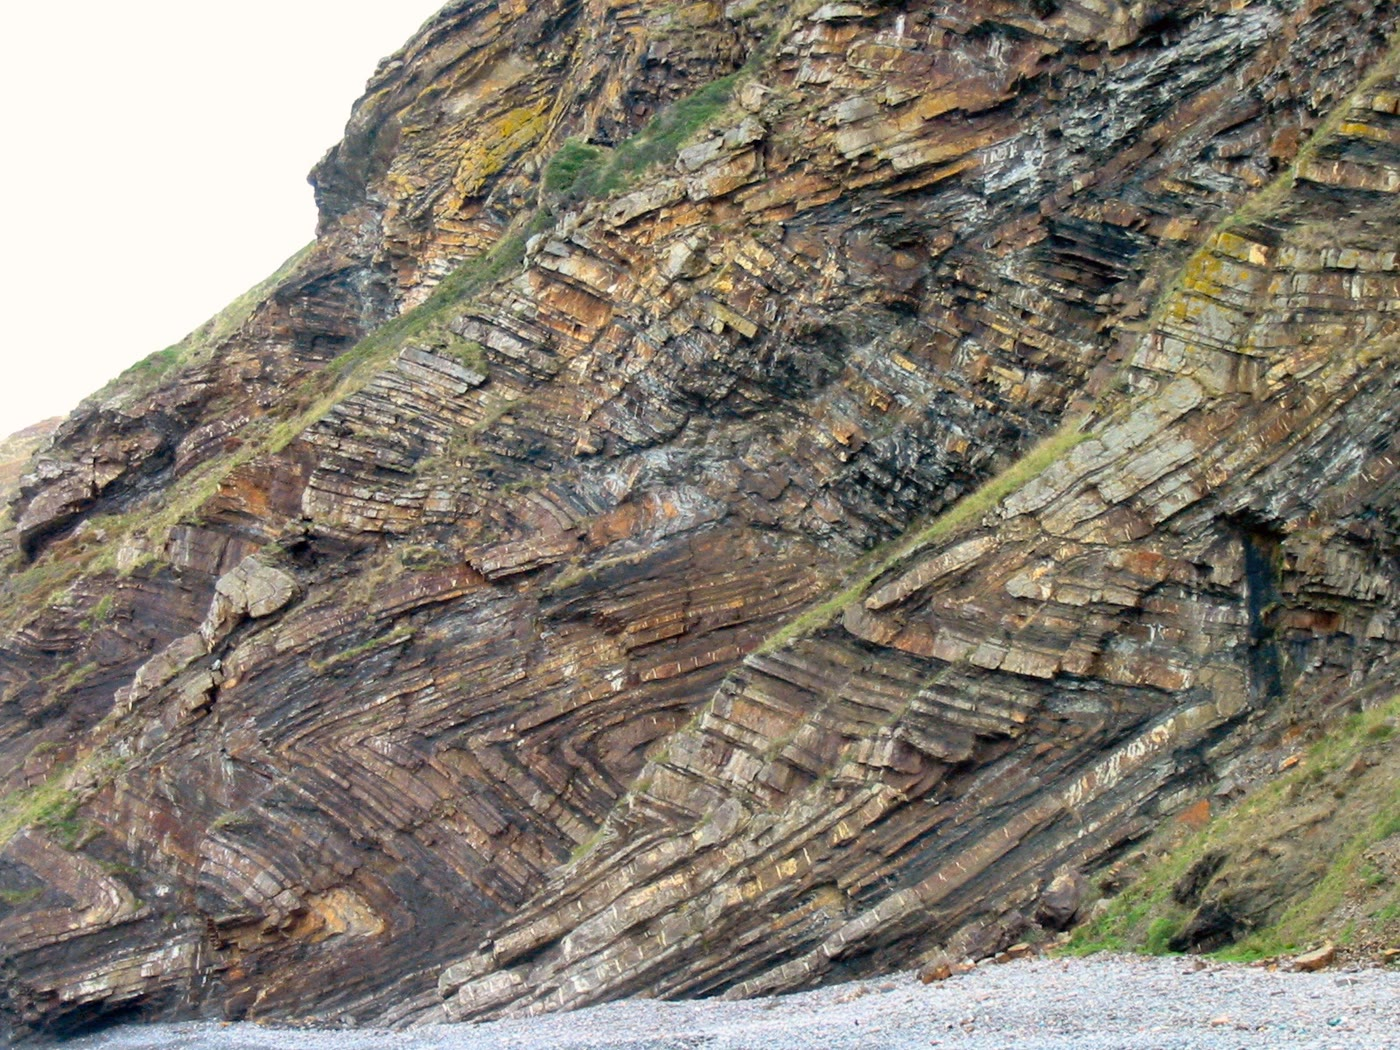
\includegraphics[width=0.78\linewidth]{images/book3/b1-chevron-folds-millook.jpg}
\par\smallskip{\small Folded beds of sandstone and shale in the cliffs at
Millook, North Cornwall: chevron \omterm{def:b1:geological-maps:fold}{folds} with nearly straight \omterm{def:b1:faults-folds-fabrics:fold-elements}{limbs} and sharp
\omterm{def:b1:faults-folds-fabrics:fold-elements}{hinges}, their \omterm{def:b1:faults-folds-fabrics:fold-elements}{axial planes} close to vertical. Photograph: Smalljim, CC~BY~3.0
(Wikimedia Commons).}
\label{fig:b1:faults-folds-fabrics:chevrons}
\end{omfigure}
% ledger: commons:millook

\section{Fabrics}\label{sec:b1:faults-folds-fabrics:fabrics}

A deformed rock is often deformed throughout, not only on a few surfaces: its
grains are flattened, turned or regrown into a common orientation, which gives
it a fabric. A planar fabric makes the rock split, a linear one makes it break
into rods.

\begin{definition}[Foliation, schistosity, slaty cleavage, axial-planar cleavage]\label{def:b1:faults-folds-fabrics:foliation}
A \emph{foliation}\index{foliation} is a planar fabric that pervades a rock:
a set of closely spaced parallel surfaces, made by aligned platy or flattened
grains or by thin layers, along which the rock splits most easily.
\emph{Schistosity}\index{schistosity} is the foliation of a schist, made by
aligned grains coarser than about \qty{1}{mm}. A \emph{cleavage}\index{cleavage
(of a rock)} is a foliation of a fine-grained rock made by its deformation;
\emph{slaty cleavage}\index{slaty cleavage} is the cleavage of a slate, made
by sheet silicates too small to be seen with the naked eye, and so closely set
that the rock can be split almost anywhere into thin sheets. An
\emph{axial-planar cleavage}\index{axial-planar
cleavage} is a cleavage parallel, or nearly parallel, to the \omterm{def:b1:faults-folds-fabrics:fold-elements}{axial planes} of
the \omterm{def:b1:geological-maps:fold}{folds} in the same rocks.
\end{definition}
% ledger: ws:fabrics

A \omterm{def:b1:faults-folds-fabrics:foliation}{foliation} forms roughly perpendicular to the direction of greatest
shortening, by the turning of platy grains, the growth of new \omterm{def:b1:rock-forming-minerals:groups}{micas}, and the
dissolution of grains on the faces that are pressed hardest. The \omterm{def:b1:faults-folds-fabrics:foliation}{cleavage} of
a slate therefore has nothing to do with the bedding of the mud: it records the
squeezing. When \omterm{def:b1:geological-maps:fold}{folds} and \omterm{def:b1:faults-folds-fabrics:foliation}{cleavage} grow in the same shortening, the \omterm{def:b1:faults-folds-fabrics:foliation}{cleavage}
lies close to the \omterm{def:b1:faults-folds-fabrics:fold-elements}{axial planes} of the \omterm{def:b1:geological-maps:fold}{folds}, and it fans slightly across them,
converging or diverging according to the strength of each layer, as the
photograph below shows.
% ledger: ws:fabrics

\begin{omfigure}
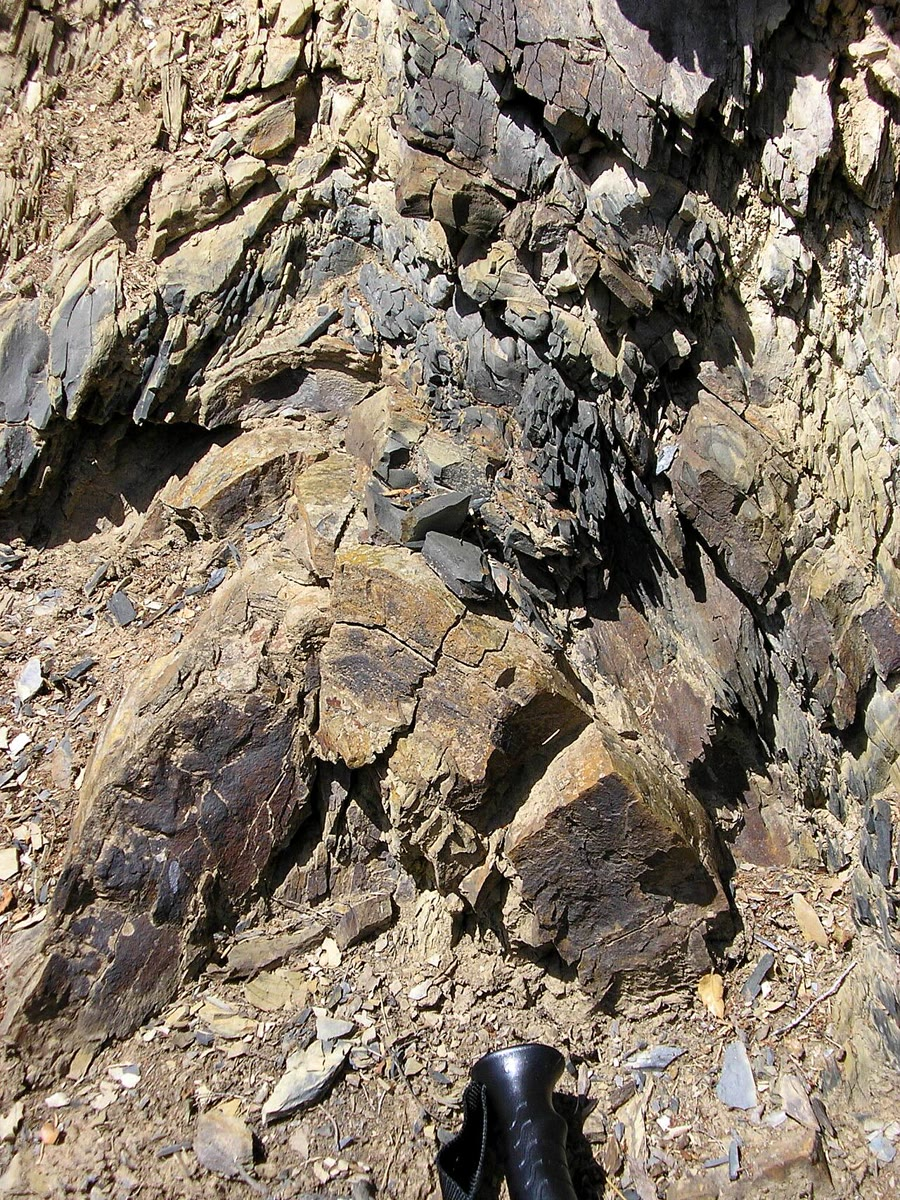
\includegraphics[height=8.2cm]{images/book3/b1-axial-planar-cleavage.jpg}
\par\smallskip{\small A small \omterm{def:b1:geological-maps:fold}{anticline} in alternating sandstone and shale of
Carboniferous age, near Potes, Cantabria. The brown sandstone beds arch over
the \omterm{def:b1:faults-folds-fabrics:fold-elements}{hinge} in the lower middle of the picture; in the dark shale above them the
\omterm{def:b1:faults-folds-fabrics:foliation}{cleavage}, a set of steep, closely spaced fractures crossing the beds, is
axial-planar: nearly parallel to the \omterm{def:b1:faults-folds-fabrics:fold-elements}{axial plane} of the \omterm{def:b1:geological-maps:fold}{fold}, it fans across
it, the fan changing from layer to layer. The handle of the walking stick is about \qty{4}{cm} across.
Photograph: Mikenorton, CC~BY-SA~3.0 (Wikimedia Commons).}
\label{fig:b1:faults-folds-fabrics:cleavage}
\end{omfigure}
% ledger: commons:axial-cleavage

\begin{definition}[Lineation, intersection lineation, stretching lineation]\label{def:b1:faults-folds-fabrics:lineation}
A \emph{lineation}\index{lineation} is a linear fabric that pervades a rock,
measured by its \omterm{def:b1:field-lab-methods-1:trend-plunge}{trend} and \omterm{def:b1:field-lab-methods-1:trend-plunge}{plunge}. An \emph{intersection
lineation}\index{intersection lineation} is the set of lines in which two
planar fabrics cut each other, such as the bedding and a \omterm{def:b1:faults-folds-fabrics:foliation}{cleavage}; a
\emph{stretching lineation}\index{stretching lineation} is made of grains or
pebbles drawn out along the direction of greatest \omterm{def:b1:stress-strain-rheology:strain}{stretch}.
\end{definition}
% ledger: ws:fabrics

\begin{proposition}[The intersection lineation of a fold]\label{prop:b1:faults-folds-fabrics:intersection}
In a \omterm{def:b1:faults-folds-fabrics:fold-elements}{cylindrical fold} with an \omterm{def:b1:faults-folds-fabrics:foliation}{axial-planar cleavage}, the \omterm{def:b1:faults-folds-fabrics:lineation}{intersection
lineation} of the bedding and the \omterm{def:b1:faults-folds-fabrics:foliation}{cleavage} is parallel to the \omterm{def:b1:faults-folds-fabrics:fold-elements}{hinge line},
everywhere on the \omterm{def:b1:geological-maps:fold}{fold}.
\end{proposition}

\begin{proof}
Every bedding surface of a \omterm{def:b1:faults-folds-fabrics:fold-elements}{cylindrical fold} contains the direction of its
axis. The \omterm{def:b1:faults-folds-fabrics:fold-elements}{axial plane} contains the \omterm{def:b1:faults-folds-fabrics:fold-elements}{hinge lines}, which are parallel to the
axis, so it contains that direction too, and so does every \omterm{def:b1:faults-folds-fabrics:foliation}{cleavage} plane
parallel to it. Two planes that are not parallel and both contain the same
direction meet along a line of that direction.
\end{proof}

The proposition is the field geologist's way to the \omterm{def:b1:field-lab-methods-1:trend-plunge}{plunge} of a \omterm{def:b1:geological-maps:fold}{fold} too large
to be seen whole: on any \omterm{def:b1:geological-maps:geological-map}{outcrop} of either limb, the lines in which the
\omterm{def:b1:faults-folds-fabrics:foliation}{cleavage} cuts the bedding give the \omterm{def:b1:faults-folds-fabrics:fold-elements}{hinge line}. The bedding and the \omterm{def:b1:faults-folds-fabrics:foliation}{cleavage}
together say more: where the \omterm{def:b1:geological-maps:fold}{fold} is, and which way up the beds are.

\begin{definition}[Vergence]\label{def:b1:faults-folds-fabrics:vergence}
The \emph{vergence}\index{vergence} of an asymmetric \omterm{def:b1:geological-maps:fold}{fold} is the horizontal
direction toward which its upper part has moved relative to its lower part:
the direction in which it is overturned or, for an \omterm{def:b1:faults-folds-fabrics:fold-classes}{inclined fold}, toward which
it leans.
\end{definition}
% ledger: ws:vergence

\begin{proposition}[Bedding and cleavage on the limbs of a fold]\label{prop:b1:faults-folds-fabrics:cleavage-bedding}
Consider a \omterm{def:b1:geological-maps:fold}{fold} with straight \omterm{def:b1:faults-folds-fabrics:fold-elements}{limbs} and an \omterm{def:b1:faults-folds-fabrics:foliation}{axial-planar cleavage}, in rocks
that were the right way up before folding, and in which both \omterm{def:b1:faults-folds-fabrics:fold-elements}{limbs} descend
from each \omterm{def:b1:geological-maps:fold}{anticline} \omterm{def:b1:faults-folds-fabrics:fold-elements}{hinge}. Seen in the profile:
\begin{enumerate}[label=(\alph*)]
  \item on a limb where the bedding and the \omterm{def:b1:faults-folds-fabrics:foliation}{cleavage} \omterm{def:b1:geological-maps:attitude}{dip} the same way, the
        bedding is the steeper of the two exactly when the limb is
        overturned;
  \item the acute rotation that turns the \omterm{def:b1:faults-folds-fabrics:foliation}{cleavage} onto the bedding has
        opposite senses on the two \omterm{def:b1:faults-folds-fabrics:fold-elements}{limbs} of a \omterm{def:b1:geological-maps:fold}{fold}; on a limb that is not
        overturned, it moves the top of the \omterm{def:b1:faults-folds-fabrics:foliation}{cleavage} horizontally toward the
        \omterm{def:b1:geological-maps:fold}{anticline} \omterm{def:b1:faults-folds-fabrics:fold-elements}{hinge} at the top of that limb.
\end{enumerate}
\end{proposition}

\begin{proof}
Look along the \omterm{def:b1:faults-folds-fabrics:fold-elements}{hinge} with the \omterm{def:b1:faults-folds-fabrics:fold-elements}{axial plane} dipping to the left at the angle
$\gamma$, $0 < \gamma \le \ang{90}$, and count angles anticlockwise from the
horizontal pointing right. The \omterm{def:b1:faults-folds-fabrics:foliation}{cleavage}, parallel to the \omterm{def:b1:faults-folds-fabrics:fold-elements}{axial plane}, runs
upward at the angle $\gamma$. At an \omterm{def:b1:geological-maps:fold}{anticline} \omterm{def:b1:faults-folds-fabrics:fold-elements}{hinge} the two \omterm{def:b1:faults-folds-fabrics:fold-elements}{limbs} leave
downward at the angles $\ang{180} + \gamma - \iota/2$ (limb~1) and
$\ang{180} + \gamma + \iota/2$ (limb~2), on either side of the \omterm{def:b1:faults-folds-fabrics:fold-elements}{axial plane},
with $\iota/2 \le \gamma$ since both descend; every limb of a train of \omterm{def:b1:geological-maps:fold}{folds}
is one of these two for the \omterm{def:b1:geological-maps:fold}{anticline} at its top. The rocks young outward,
away from the core of the \omterm{def:b1:geological-maps:fold}{anticline}, along the normal to the limb that points
away from the \omterm{def:b1:faults-folds-fabrics:fold-elements}{axial plane}.

Limb~1 goes down to the left: it \omterm{def:b1:geological-maps:attitude}{dips} to the left at $\gamma - \iota/2$, less
steeply than the \omterm{def:b1:faults-folds-fabrics:foliation}{cleavage}. Its outward normal, at $\ang{90} + \gamma -
\iota/2$, points upward: it is the right way up. Running upward, it makes the
angle $\gamma - \iota/2$, so the acute rotation from the \omterm{def:b1:faults-folds-fabrics:foliation}{cleavage} to the bedding
is clockwise, through $\iota/2$: the top of the \omterm{def:b1:faults-folds-fabrics:foliation}{cleavage} moves to the right,
where the \omterm{def:b1:faults-folds-fabrics:fold-elements}{hinge} is, since the limb leaves the \omterm{def:b1:faults-folds-fabrics:fold-elements}{hinge} toward the left.

Limb~2 makes the angle $\gamma + \iota/2$ with the horizontal, upward. If
$\gamma + \iota/2 > \ang{90}$, it goes down to the right and \omterm{def:b1:geological-maps:attitude}{dips} to the
right, opposite to the \omterm{def:b1:faults-folds-fabrics:foliation}{cleavage}; its outward normal, at $\ang{270} + \gamma +
\iota/2$, has the upward component $-\cos(\gamma + \iota/2) > 0$: it is the
right way up. If $\gamma + \iota/2 < \ang{90}$, it goes down to the left,
dipping to the left at $\gamma + \iota/2$, more steeply than the \omterm{def:b1:faults-folds-fabrics:foliation}{cleavage}, and
the same component is negative: the limb is overturned. In both cases the acute
rotation from the \omterm{def:b1:faults-folds-fabrics:foliation}{cleavage} to the bedding is anticlockwise, through $\iota/2$,
and moves the top of the \omterm{def:b1:faults-folds-fabrics:foliation}{cleavage} to the left; when the limb is the right way
up it leaves the \omterm{def:b1:faults-folds-fabrics:fold-elements}{hinge} toward the right, so the \omterm{def:b1:faults-folds-fabrics:fold-elements}{hinge} is to the left. \omterm{def:b1:faults-folds-fabrics:fold-elements}{Limbs}
that \omterm{def:b1:geological-maps:attitude}{dip} the same way as the \omterm{def:b1:faults-folds-fabrics:foliation}{cleavage} are thus limb~1, less steep, and an
overturned limb~2, steeper, which is (a); the senses are clockwise on limb~1
and anticlockwise on limb~2, which is (b).
\end{proof}

The sense of the rotation thus changes at every \omterm{def:b1:faults-folds-fabrics:fold-elements}{hinge}, \omterm{def:b1:geological-maps:fold}{anticline} or \omterm{def:b1:geological-maps:fold}{syncline}.
A geologist who records it along a traverse finds the \omterm{def:b1:faults-folds-fabrics:fold-elements}{hinges} of \omterm{def:b1:geological-maps:fold}{folds} too
large to see in one \omterm{def:b1:geological-maps:geological-map}{outcrop} where the sense changes, and the overturned \omterm{def:b1:faults-folds-fabrics:fold-elements}{limbs}
where the bedding is steeper than the \omterm{def:b1:faults-folds-fabrics:foliation}{cleavage}; the word \omterm{def:b1:faults-folds-fabrics:vergence}{vergence} is also used
for this sense of rotation, and the reversals of \omterm{def:b1:geological-maps:fold}{minor-fold} \omterm{def:b1:faults-folds-fabrics:vergence}{vergence} are
mapped in the same way to find the \omterm{def:b1:faults-folds-fabrics:fold-elements}{hinges} of major \omterm{def:b1:geological-maps:fold}{folds}: the small \omterm{def:b1:geological-maps:fold}{folds} on
the two \omterm{def:b1:faults-folds-fabrics:fold-elements}{limbs} of a large one have opposite asymmetries, and its axial trace
runs between them.
% ledger: ws:vergence, ws:fold-elements

\begin{omfigure}
\begin{tikzpicture}[>={Stealth[length=5pt]}, font=\small]
% a train of chevron folds seen along the hinge (north into the page, east to the right):
% axial planes dipping 60 deg to the west, interlimb angle 40 deg; long limbs dip 40 deg W
% (the right way up), short limbs 80 deg W (overturned). Short limb: from an anticline hinge H_k,
% length s along 260 deg to the syncline hinge S_k; long limb back up along 40 deg to H_{k+1},
% so that all anticline hinges are level, a wavelength w apart.
% Five bedding surfaces, repeated along the axial direction (similar folds); cleavage parallel to it.
\def\s{2.6}
\pgfmathsetmacro{\sx}{\s*cos(260)}\pgfmathsetmacro{\sy}{\s*sin(260)}
\pgfmathsetmacro{\w}{\sx - \sy/tan(40)}
\pgfmathsetmacro{\hx}{0.62*cos(60)}\pgfmathsetmacro{\hy}{0.62*sin(60)}
\newcommand{\surface}[1]{%
  (-\w+#1*\hx, #1*\hy) \foreach \k in {-1,0,1,2,3} { -- ({\k*\w+\sx+#1*\hx}, {\sy+#1*\hy}) -- ({(\k+1)*\w+#1*\hx}, {#1*\hy}) }}
\begin{scope}
  \clip (0.35,-3.3) rectangle (10.0,2.95);
  \begin{scope}
    \clip \surface{0} -- (12,6) -- (-4,6) -- cycle;
    \clip \surface{4} -- (12,-6) -- (-4,-6) -- cycle;
    \fill[omLithSand!45] (-4,-6) rectangle (12,6);
    \fill[omLithShale!40] \surface{2} -- (12,6) -- (-4,6) -- cycle;
    \fill[omLithSand!45] \surface{3} -- (12,6) -- (-4,6) -- cycle;
    \foreach \c in {-8.0,-7.78,...,13.0} {
      \draw[omDef!85, line width=0.35pt] ({\c-6*cot(60)},-6) -- ({\c+6*cot(60)},6);
    }
  \end{scope}
  \foreach \j in {0,1,2,3,4} { \draw[line width=0.75pt, line join=round] \surface{\j}; }
\end{scope}
% axial traces through the anticline hinges, and labels
\foreach \k in {1,2,3} {
  \draw[omThm, dashed, line width=0.6pt] ({\k*\w-0.5*cos(60)},{-0.5*sin(60)}) -- ({\k*\w+3.6*cos(60)},{3.6*sin(60)});
  \node[omThm, font=\scriptsize, anchor=south] at ({\k*\w+3.6*cos(60)},{3.6*sin(60)}) {anticline};
}
\foreach \k in {1,2,3} { \node[omThm, font=\scriptsize, anchor=north] at ({\k*\w+\sx},{\sy-0.15}) {syncline}; }
\end{tikzpicture}
\par\smallskip{\small A train of chevron \omterm{def:b1:geological-maps:fold}{folds} overturned to the right, in
profile, with an \omterm{def:b1:faults-folds-fabrics:foliation}{axial-planar cleavage} (thin blue lines), drawn to scale: \omterm{def:b1:faults-folds-fabrics:fold-elements}{axial
planes} dipping \ang{60} to the left, \omterm{def:b1:faults-folds-fabrics:fold-elements}{interlimb angle} \ang{40}. The long \omterm{def:b1:faults-folds-fabrics:fold-elements}{limbs}
\omterm{def:b1:geological-maps:attitude}{dip} \ang{40} to the left, less steeply than the \omterm{def:b1:faults-folds-fabrics:foliation}{cleavage}, and are the right
way up; the short \omterm{def:b1:faults-folds-fabrics:fold-elements}{limbs} \omterm{def:b1:geological-maps:attitude}{dip} \ang{80} to the left, more steeply than the
\omterm{def:b1:faults-folds-fabrics:foliation}{cleavage}, and are overturned. Turning the \omterm{def:b1:faults-folds-fabrics:foliation}{cleavage} onto the bedding through
the acute angle is clockwise on every long limb and anticlockwise on every
short limb. The \omterm{def:b1:geological-maps:fold}{folds} verge to the right.}
\label{fig:b1:faults-folds-fabrics:vergence}
\end{omfigure}

\section{Microstructures}\label{sec:b1:faults-folds-fabrics:micro}

Under the microscope, the deformation of a rock shows in its grains. A grain
of quartz bent by the slow gliding of its crystal lattice no longer goes into
extinction all at once between \omterm{def:b1:field-lab-methods-1:microscope}{crossed polars}: as the stage turns, a dark band
sweeps across it, because its parts point in slightly different directions.
This undulose extinction (\cref{ch:b1:optical-mineralogy}) grows stronger as
a shear zone is approached, because defects pile up in the crystal lattice.
Where water is present, grains dissolve on the faces where they are pressed
hardest and the dissolved matter is deposited where the stress is lower, or
carried away: this pressure solution shortens rocks at low temperature and
builds many \omterm{def:b1:faults-folds-fabrics:foliation}{cleavages}. At higher temperature, the strained grains are
replaced, while the deformation goes on, by new, smaller and unstrained ones,
first along the old grain boundaries: dynamic recrystallisation, which shrinks
the grain size and makes \omterm{def:b1:faults-folds-fabrics:fault-rocks}{mylonites}. The shapes of deformed grains and of the \omterm{def:b1:rock-forming-minerals:mineral}{minerals} that grow in
their shadows also show which way a shear zone moved; these shear-sense
indicators, and the mechanisms themselves, belong to the Year~3 volume.
% ledger: ws:microstructures, ws:fabrics

\section{Exercises}

\begin{exercise}[$\star$]\label{exo:b1:faults-folds-fabrics:1}
Name each fault from the \omterm{def:b1:faults-folds-fabrics:fault-elements}{rake} of its \omterm{def:b1:faults-folds-fabrics:fault-elements}{slip vector}, the plane dipping \ang{60}:
(a) $r = \ang{-90}$; (b) $r = \ang{85}$; (c) $r = 0$; (d) $r = \ang{180}$;
(e) $r = \ang{-40}$. (f) What would (b) be called if its \omterm{def:b1:geological-maps:attitude}{dip} were \ang{25}?
% ledger: ar:rake, usgs:fault-types
\end{exercise}

\begin{exercise}[$\star$]\label{exo:b1:faults-folds-fabrics:2}
A \omterm{def:b1:faults-folds-fabrics:fault-types}{normal fault} \omterm{def:b1:geological-maps:attitude}{dips} \ang{55}; its slip is pure dip-slip, with a \omterm{def:b1:faults-folds-fabrics:fault-elements}{net slip} of
\qty{300}{m}. Compute its \omterm{def:b1:cross-sections:throw}{throw} and its \omterm{def:b1:cross-sections:throw}{heave}.
\end{exercise}

\begin{exercise}[$\star$]\label{exo:b1:faults-folds-fabrics:3}
Give the \omterm{def:b1:faults-folds-fabrics:fold-elements}{interlimb angle} and the class of each \omterm{def:b1:faults-folds-fabrics:fold-classes}{upright fold}, whose \omterm{def:b1:faults-folds-fabrics:fold-elements}{limbs} \omterm{def:b1:geological-maps:attitude}{dip}
in opposite directions: (a) \omterm{def:b1:faults-folds-fabrics:fold-elements}{limbs} dipping \ang{35} and \ang{35}; (b) \ang{70}
and \ang{75}; (c) \ang{85} and \ang{88}.
% ledger: ws:fold-classes
\end{exercise}

\begin{exercise}[$\star$]\label{exo:b1:faults-folds-fabrics:4}
A sandstone has the \omterm{def:b1:stress-strain-rheology:coulomb}{angle of internal friction} \ang{35}. Following Anderson's
theory, at what angles do its \omterm{def:b1:faults-folds-fabrics:fault-types}{normal faults} and its \omterm{def:b1:faults-folds-fabrics:fault-types}{thrust faults} \omterm{def:b1:geological-maps:attitude}{dip}? What
angle do two conjugate \omterm{def:b1:faults-folds-fabrics:fault-types}{strike-slip faults} make with each other?
\end{exercise}

\begin{exercise}[$\star\star$]\label{exo:b1:faults-folds-fabrics:5}
A fault has the \omterm{def:b1:geological-maps:attitude}{attitude} $090/50$, and \omterm{def:b1:faults-folds-fabrics:fault-rocks}{slickenlines} of \omterm{def:b1:faults-folds-fabrics:fault-elements}{rake} \ang{-30} on it;
the \omterm{def:b1:faults-folds-fabrics:fault-elements}{net slip} is \qty{400}{m}. (a) Compute the strike-slip and dip-slip
components, the \omterm{def:b1:cross-sections:throw}{throw} and the \omterm{def:b1:cross-sections:throw}{heave}. (b) Write the \omterm{def:b1:faults-folds-fabrics:fault-elements}{slip vector} in east, north
and up components, and give its \omterm{def:b1:field-lab-methods-1:trend-plunge}{trend} and \omterm{def:b1:field-lab-methods-1:trend-plunge}{plunge}. (c) Name the fault.
\end{exercise}

\begin{exercise}[$\star\star$]\label{exo:b1:faults-folds-fabrics:6}
Two vertical \omterm{def:b1:faults-folds-fabrics:fault-types}{strike-slip faults} of the same age \omterm{def:b1:geological-maps:attitude}{strike} $020$ and $080$.
(a) Following Anderson, give the directions of $\sigma_1$, $\sigma_2$ and
$\sigma_3$, and the \omterm{def:b1:stress-strain-rheology:coulomb}{angle of internal friction} of the rock. (b) Which fault is
\omterm{def:b1:faults-folds-fabrics:fault-types}{dextral} and which \omterm{def:b1:faults-folds-fabrics:fault-types}{sinistral}? Argue from the shortening along $\sigma_1$.
\end{exercise}

\begin{exercise}[$\star\star$]\label{exo:b1:faults-folds-fabrics:7}
The two \omterm{def:b1:faults-folds-fabrics:fold-elements}{limbs} of a \omterm{def:b1:faults-folds-fabrics:fold-elements}{cylindrical fold} have the \omterm{def:b1:geological-maps:attitude}{attitudes} $120/40$ and $260/30$.
With \cref{prop:b1:faults-folds-fabrics:hinge}, find the \omterm{def:b1:field-lab-methods-1:trend-plunge}{trend} and \omterm{def:b1:field-lab-methods-1:trend-plunge}{plunge} of
its \omterm{def:b1:faults-folds-fabrics:fold-elements}{hinge line}, its \omterm{def:b1:faults-folds-fabrics:fold-elements}{interlimb angle} and its class.
\end{exercise}

\begin{exercise}[$\star\star$]\label{exo:b1:faults-folds-fabrics:8}
At an \omterm{def:b1:geological-maps:geological-map}{outcrop}, the bedding has the \omterm{def:b1:geological-maps:attitude}{attitude} $040/30$ and an \omterm{def:b1:faults-folds-fabrics:foliation}{axial-planar
cleavage} the \omterm{def:b1:geological-maps:attitude}{attitude} $160/80$. Find the \omterm{def:b1:field-lab-methods-1:trend-plunge}{trend} and \omterm{def:b1:field-lab-methods-1:trend-plunge}{plunge} of the \omterm{def:b1:faults-folds-fabrics:lineation}{intersection
lineation}. What does it tell about the \omterm{def:b1:geological-maps:fold}{fold}?
\end{exercise}

\begin{exercise}[$\star\star$]\label{exo:b1:faults-folds-fabrics:9}
A vertical fault \omterm{def:b1:geological-maps:attitude}{strikes} east--west. A vertical dyke striking north--south
crosses it; north of the fault the dyke is found \qty{350}{m} east of where
it is south of the fault. (a) Is the fault \omterm{def:b1:faults-folds-fabrics:fault-types}{dextral} or \omterm{def:b1:faults-folds-fabrics:fault-types}{sinistral}? (b) If the
\omterm{def:b1:faults-folds-fabrics:fault-rocks}{slickenlines} are horizontal, what is the \omterm{def:b1:faults-folds-fabrics:fault-elements}{net slip}? (c) If instead they \omterm{def:b1:field-lab-methods-1:trend-plunge}{plunge}
\ang{20} to the east, what are the \omterm{def:b1:faults-folds-fabrics:fault-elements}{net slip} and the vertical component of the
slip, and which block went down?
\end{exercise}

\begin{exercise}[$\star\star\star$]\label{exo:b1:faults-folds-fabrics:10}
A fault with no \omterm{def:b1:stress-strain-rheology:coulomb}{cohesion} and the friction coefficient $\mu$ makes the angle
$\theta$ with $\sigma_1$. (a) Show that it slips when the effective \omterm{def:b1:stress-strain-rheology:principal}{principal
stresses} reach the ratio
\[
  \frac{\sigma_1'}{\sigma_3'} = \frac{1 + \mu\cot\theta}{1 - \mu\tan\theta} .
\]
(b) With $\mu = 0.6$ and $\sigma_1$ vertical, compute the ratio for \omterm{def:b1:faults-folds-fabrics:fault-types}{normal
faults} dipping \ang{60}, \ang{45} and \ang{35}. (c) Show that a \omterm{def:b1:faults-folds-fabrics:fault-types}{normal fault}
dipping less than a certain angle can never slip, and compute that angle.
(d) For $\mu = 0.6$ and $\mu = 0.85$, give the \omterm{def:b1:geological-maps:attitude}{dips} of the best-oriented
normal and \omterm{def:b1:faults-folds-fabrics:fault-types}{thrust faults}.
\end{exercise}

\begin{exercise}[$\star\star\star$]\label{exo:b1:faults-folds-fabrics:11}
Along an east--west traverse across chevron \omterm{def:b1:geological-maps:fold}{folds} whose \omterm{def:b1:faults-folds-fabrics:fold-elements}{hinges} \omterm{def:b1:field-lab-methods-1:trend-plunge}{trend} north,
an \omterm{def:b1:faults-folds-fabrics:foliation}{axial-planar cleavage} \omterm{def:b1:geological-maps:attitude}{dips} \ang{60} to the west everywhere. The bedding
\omterm{def:b1:geological-maps:attitude}{dips} \ang{40} W at station A, \ang{80} W at station B and \ang{40} W at
station C, from west to east, in rocks that were the right way up before
folding. (a) Which station is on an overturned limb? (b) In which sense does
the \omterm{def:b1:faults-folds-fabrics:foliation}{cleavage} turn onto the bedding at each station, seen looking north?
(c) Where are the \omterm{def:b1:faults-folds-fabrics:fold-elements}{hinges}, and which are \omterm{def:b1:geological-maps:fold}{anticlines}? (d) Find the \omterm{def:b1:faults-folds-fabrics:fold-elements}{interlimb
angle} and the \omterm{def:b1:geological-maps:attitude}{attitude} of the \omterm{def:b1:faults-folds-fabrics:fold-elements}{axial planes}, and say which way the \omterm{def:b1:geological-maps:fold}{folds}
verge.
\end{exercise}

\begin{exercise}[$\star\star\star$]\label{exo:b1:faults-folds-fabrics:12}
A layer of length $L_0$ is folded into a train of symmetric chevron \omterm{def:b1:geological-maps:fold}{folds} of
\omterm{def:b1:faults-folds-fabrics:fold-elements}{interlimb angle} $\iota$, with its length unchanged. (a) Show that its length
measured across the \omterm{def:b1:geological-maps:fold}{folds} becomes $L_0\sin(\iota/2)$. (b) What shortening do
chevron \omterm{def:b1:geological-maps:fold}{folds} of \omterm{def:b1:faults-folds-fabrics:fold-elements}{interlimb angle} \ang{60} represent? (c) What \omterm{def:b1:faults-folds-fabrics:fold-elements}{interlimb angle}
corresponds to a shortening of \qty{30}{\percent}? (d) A train of \omterm{def:b1:faults-folds-fabrics:fold-classes}{upright
folds} with \omterm{def:b1:faults-folds-fabrics:fold-elements}{limbs} dipping \ang{12}: what shortening?
\end{exercise}

\section{Problem: The Varden Hills' structures, measured}

\begin{problem}[{Weekend problem --- the anticline and the normal fault of
the Varden Hills, from the attitudes of their planes to the slip on the
fault}]
\label{pb:b1:faults-folds-fabrics:1}
% values: calc/ch17.py; region: figdata/shared/region.py (limbs, plunge, fault)
The Varden Hills are folded into an \omterm{def:b1:geological-maps:fold}{anticline}, whose axis runs north--south
at $x = \qty{3.5}{km}$, and a \omterm{def:b1:geological-maps:fold}{syncline} \qty{4}{km} to the east of it; both
have planar \omterm{def:b1:faults-folds-fabrics:fold-elements}{limbs}. A field survey measured the bedding on the east limb of
the \omterm{def:b1:geological-maps:fold}{anticline} as $080.7/12.2$ and on its west limb as $279.3/12.2$. The cover
is cut by a \omterm{def:b1:faults-folds-fabrics:fault-types}{normal fault} of \omterm{def:b1:geological-maps:attitude}{attitude} $120/60$, whose \omterm{def:b1:faults-folds-fabrics:fault-elements}{hanging wall} moved down
the \omterm{def:b1:geological-maps:attitude}{dip}, with a \omterm{def:b1:cross-sections:throw}{throw} of \qty{200}{m}. Give angles to \ang{0.1} and lengths to
\qty{0.1}{m}.

\medskip
\noindent\textbf{Part I --- The limbs.}
\begin{enumerate}
  \item Write the upward unit normals $\mathbf n_1$ (east limb) and
        $\mathbf n_2$ (west limb) in east, north and up components.
  \item Compute $\mathbf n_1\cdot\mathbf n_2$ and the angle between the
        normals.
  \item Deduce the \omterm{def:b1:faults-folds-fabrics:fold-elements}{interlimb angle} of the \omterm{def:b1:geological-maps:fold}{anticline}.
  \item Classify the \omterm{def:b1:geological-maps:fold}{anticline} by its \omterm{def:b1:faults-folds-fabrics:fold-elements}{interlimb angle}.
  \item The two \omterm{def:b1:faults-folds-fabrics:fold-elements}{limbs} \omterm{def:b1:geological-maps:attitude}{dip} \ang{12.2}. Why is the \omterm{def:b1:faults-folds-fabrics:fold-elements}{interlimb angle} not exactly
        $\ang{180} - 2\times\ang{12.2}$? Compute the \omterm{def:b1:cross-sections:apparent-dip}{apparent dip} of either
        limb in an east--west vertical section.
  \item The \omterm{def:b1:geological-maps:fold}{syncline} shares the east limb of the \omterm{def:b1:geological-maps:fold}{anticline}, and its own east
        limb is parallel to the \omterm{def:b1:geological-maps:fold}{anticline}'s west limb. What is its \omterm{def:b1:faults-folds-fabrics:fold-elements}{interlimb
        angle}?
\end{enumerate}

\medskip
\noindent\textbf{Part II --- The hinge line and the axial plane.}
\begin{enumerate}[resume]
  \item Compute $\mathbf n_1\times\mathbf n_2$, and the \omterm{def:b1:field-lab-methods-1:trend-plunge}{trend} and \omterm{def:b1:field-lab-methods-1:trend-plunge}{plunge} of
        the \omterm{def:b1:faults-folds-fabrics:fold-elements}{hinge line}.
  \item Give the \omterm{def:b1:geological-maps:attitude}{attitude} of the \omterm{def:b1:faults-folds-fabrics:fold-elements}{axial plane}. Is the \omterm{def:b1:geological-maps:fold}{anticline} upright,
        inclined or recumbent?
  \item Give the full description of the \omterm{def:b1:geological-maps:fold}{fold}: tightness, \omterm{def:b1:geological-maps:attitude}{attitude} of the
        \omterm{def:b1:faults-folds-fabrics:fold-elements}{axial plane}, \omterm{def:b1:field-lab-methods-1:trend-plunge}{plunge}.
  \item On the \omterm{def:b1:geological-maps:geological-map}{geological map} of \cref{ch:b1:geological-maps}, which way do
        the \omterm{def:b1:geological-maps:geological-map}{outcrops} of the \omterm{def:b1:geological-maps:fold}{anticline} close, and what crops out in its core?
  \item The shale of the cover carries an \omterm{def:b1:faults-folds-fabrics:foliation}{axial-planar cleavage}. Give its
        \omterm{def:b1:geological-maps:attitude}{attitude}, and the \omterm{def:b1:field-lab-methods-1:trend-plunge}{trend} and \omterm{def:b1:field-lab-methods-1:trend-plunge}{plunge} of its \omterm{def:b1:faults-folds-fabrics:lineation}{intersection lineation} on
        the east limb.
  \item On the east limb, in which sense does the \omterm{def:b1:faults-folds-fabrics:foliation}{cleavage} turn onto the
        bedding, seen looking north, and on which side is the \omterm{def:b1:geological-maps:fold}{anticline} \omterm{def:b1:faults-folds-fabrics:fold-elements}{hinge}?
\end{enumerate}

\medskip
\noindent\textbf{Part III --- The fault and the stresses.}
\begin{enumerate}[resume]
  \item Give the \omterm{def:b1:geological-maps:attitude}{strike} of the fault by the right-hand rule, and say on which
        side of its trace the \omterm{def:b1:faults-folds-fabrics:fault-elements}{hanging wall} lies.
  \item Which principal stress was vertical when the fault formed, according
        to Anderson?
  \item Give the directions of the two horizontal \omterm{def:b1:stress-strain-rheology:principal}{principal stresses}.
  \item What \omterm{def:b1:stress-strain-rheology:coulomb}{angle of internal friction} does the \omterm{def:b1:geological-maps:attitude}{dip} imply? What \omterm{def:b1:stress-strain-rheology:coulomb}{coefficient
        of internal friction}?
  \item Give the \omterm{def:b1:geological-maps:attitude}{attitude} of the conjugate set of faults that the same
        stresses could have made, and the angle between the two sets.
  \item Would the fault be best oriented to slip again under the same regime,
        with Byerlee's friction of 0.85?
\end{enumerate}

\medskip
\noindent\textbf{Part IV --- The slip.}
\begin{enumerate}[resume]
  \item Give the \omterm{def:b1:faults-folds-fabrics:fault-elements}{rake} of the \omterm{def:b1:faults-folds-fabrics:fault-elements}{slip vector}, and its \omterm{def:b1:field-lab-methods-1:trend-plunge}{trend} and \omterm{def:b1:field-lab-methods-1:trend-plunge}{plunge}.
  \item Write the unit vector of the slip in east, north and up components.
  \item Compute the \omterm{def:b1:cross-sections:throw}{heave} of the fault.
  \item Compute the east and north components of the horizontal displacement
        of the \omterm{def:b1:faults-folds-fabrics:fault-elements}{hanging wall}.
  \item Check that the \omterm{def:b1:faults-folds-fabrics:fault-elements}{net slip} $L$, the \omterm{def:b1:cross-sections:throw}{throw} $h$ and the \omterm{def:b1:cross-sections:throw}{heave} $e$ satisfy
        $L^2 = h^2 + e^2$, and explain why.
  \item To the nearest metre, what is the \omterm{def:b1:faults-folds-fabrics:fault-elements}{net slip} on the Varden fault?
\end{enumerate}
\end{problem}
